\documentclass[11pt,a4paper,twoside,openright]{report}

\usepackage[dvips]{graphicx}
\usepackage{tabularx}
\usepackage{subfigure}
\usepackage{afterpage}
\usepackage{amsmath,amssymb}
\usepackage{rotating}
\usepackage{fancyhdr}
\usepackage[scriptsize]{caption}
\hyphenation{a-gen-tiz-za-zio-ne}

\setlength{\paperwidth}{16cm}
\setlength{\paperheight}{24cm}
\setlength{\oddsidemargin} {2. cm}
\setlength{\evensidemargin} {2. cm}
\addtolength{\oddsidemargin} {-0.4 cm}
\addtolength{\evensidemargin} {-0.4 cm}
\linespread{1.1}

\usepackage[italian]{babel}
\usepackage[latin1]{inputenc}
\renewcommand{\captionfont}{\normalfont \sffamily \itshape \small}

\pagestyle{empty}
%\usepackage[colorlinks=true,italian,breaklinks,setpagesize=false]{hyperref}
\usepackage{hyperref}
\hypersetup{
			hidelinks,
			italian,
			breaklinks,
			setpagesize=false}

\begin{document}
\thispagestyle{empty}
%\begin{titlepage}
\vspace*{-1.5cm} \bfseries{
\begin{center}
  \large
  POLITECNICO DI MILANO\\
  \normalsize
  Corso di Laurea \textbf{MAGISTRALE} in Ingegneria Informatica\\
  Dipartimento di Elettronica, Informazione e Bioingegneria\\
  \begin{figure}[htbp]
    \begin{center}
      
\includegraphics[width=3.5cm]{./pictures/logopm}
%	
\psfig{file=./pictures/logopm.jpg,width=3.5cm}
    \end{center}
  \end{figure}
  \vspace*{0.3cm} \LARGE



  \textbf{TITOLO DELLA TESI}\\



%  \vspace*{.75truecm} \large
%  AI \& R Lab \\
%  Laboratorio di Intelligenza Artificiale \\
%  e Robotica del Politecnico di Milano
\end{center}
\vspace*{3.0cm} \large
\begin{flushleft}


  Relatore: Prof. Pier Luca Lanzi \\
  Correlatore: \dots

\end{flushleft}
\vspace*{1.0cm}
\begin{flushright}


  Tesi di Laurea di:\\ Nicola Padovano, matricola \dots \\ 
		       Elia Polo, matricola 760649 \\


\end{flushright}
\vspace*{0.5cm}
\begin{center}



  Anno Accademico 2013-2014
\end{center} \clearpage
}

\thispagestyle{empty} \normalfont \cleardoublepage
%\include{dedica}
%\thispagestyle{empty}  \cleardoublepage
\pagenumbering{arabic}
\newpage
\chapter*{Sommario}

\addcontentsline{toc}{chapter}{Sommario}

Il sommario deve contenere 3 o 4 frasi tratte dall'introduzione di cui la prima inquadra l'area dove si svolge il lavoro (eventualmente la seconda inquadra la sottoarea pi\`u specifica del lavoro), la seconda o la terza frase dovrebbe iniziare con le parole ``Lo scopo della tesi \`e \dots'' e infine la terza o quarta frase riassume brevemente l'attivit\`a  svolta, i risultati ottenuti ed eventuali valutazioni di questi.

\vspace{0.5cm}
\noindent NB: se il relatore effettivo \`e interno al Politecnico di Milano nel frontespizio si scrive Relatore, se vi \`e la collaborazione di un altro studioso lo si riporta come Correlatore come sopra. Nel caso il relatore effettivo sia esterno si scrive Relatore esterno e poi bisogna inserire anche il Relatore interno. Nel caso il relatore sia un ricercatore allora il suo Nome COGNOME dovr\`a  essere preceduto da Ing. oppure Dott., a seconda dei casi.

\thispagestyle{empty} \vspace*{.75truecm} \cleardoublepage
%\include{ringraziamenti}
%\thispagestyle{empty} \vspace*{.75truecm} \normalfont \cleardoublepage
\pagestyle{plain}\renewcommand{\chaptermark}[1]{\markboth{\chaptername\ \thechapter.\ #1}{}} 
\renewcommand{\sectionmark}[1]{\markright{\thesection.\ #1}}         
\fancyhead[LE,RO]{\bfseries\thepage}    
                                        
\fancyhead[RE]{\bfseries\leftmark}    
\fancyhead[LO]{\bfseries\rightmark}     
\renewcommand{\headrulewidth}{0.3pt} 

\chapter{Introduzione}
\label{Introduzione}
\thispagestyle{empty}
I servizi informatici che utilizziamo quotidianamente---dalla posta elettronica ai motori di ricerca, dai \textit{social network} ai giochi online---sono sempre pi� spesso gratuiti e si sostengono grazie alla pubblicit�: direttamente, esponendo contenuto promozionale, o indirettamente, dalla valorizzazione delle nostre informazioni personali a fini pubblicitari. Per massimizzare l'efficacia della pubblicit�, ossia trasformare l'utente in cliente, � tuttavia essenziale identificare i gusti e gli interessi dell'individuo che si ha di fronte, e proporgli inserzioni personalizzate che rispondano o addirittura anticipino una sua reale esigenza. Nell'era odierna dei Big Data, una moltitudine di nuovi dati su masse di
utenti \`e prontamente accessibile: l'attivit\`a sui siti internet, il profilo sui
social network, le relazioni sociali e il sentiment (le opinioni, i gusti e l'affiliazione a idee, prodotti, marchi, individui).  Ci\`o ha portato a ridefinire l'idea stessa della segmentazione di mercato---la disaggregazione dei clienti in gruppi omogenei per esigenze e comportamento di acquisto---per cui la ripartizione in aree geografiche, demografiche e psicografiche \`e obsoleta o insufficiente. Queste realt\`a, la necessit\`a di profilare gli utenti e il diluvio di informazione grezza che ciascuno di noi divulga su internet, sono fortemente sinergiche, ma richiedono una laboriosa raffinazione per poter essere impiegate nel marketing.\\
La segmentazione di mercato pu� essere costruita a partire dalle divisioni identificate mediante tecniche di clustering, un processo che organizza una popolazione in gruppi formati da individui affini. Un esperto dovr\`a poi attribuire un significato (profiling) a tali gruppi, comporli per caratterizzare una tipologia di consumatori tramite le variabili usate per il clustering nonch� le caratteristiche demografiche, geografiche e comportamentali degli individui, al fine di elaborare una strategia di marketing peculiare per ciascun segmento.\\
Pertanto, per avvalersi dell'informazione proveniente dai social network a fini commerciali, � necessario definire una metodologia per il clustering di grandi volumi di dati: profili utente con un elevato numero di attributi e talvolta arricchiti da una tela di relazioni sociali. Lo scopo della tesi � realizzare un framework per il clustering di vasti grafi con attributi, che sia di supporto al processo di segmentazione.\\
Questo lavoro � stato motivato dall'esigenza di Neosperience, una azienda che offre servizi di marketing e \textit{customer experience}, di valorizzare i dati degli utenti---sotto forma di profili Facebook, Twitter e Foursquare---raccolti tramite la propria piattaforma Engage. Il lavoro � iniziato dall'analisi degli algoritmi esistenti in letteratura che potessero adattarsi al tipo, dimensione e volume dei dati su cui avremmo operato. In seguito sono stati raccolti i dati, una ampia collezione di profili Facebook, composti da informazioni di profilo, preferenze (\textit{like}) e connessioni sociali (\textit{friend}). Una volta reperito il codice degli algoritmi, i dati sono stati ripuliti e preparati per le tecniche di clustering selezionate. Dall'esecuzione degli algoritmi su svariati campioni del dataset completo abbiamo potuto evidenziare i punti di forza e debolezza di ciascun approccio. Tramite la misurazione di indici di qualit�, siamo in grado di suggerire qual � la miglior parametrizzazione di ciascun algoritmo su un dataset in input e di svolgere una analisi comparativa sulle prestazioni delle diverse tecniche.

\section{Contesto del lavoro}
\label{sec:contesto}
Il clustering � un processo che, partendo da una definizione di similarit� e una popolazione, produce una suddivisione degli individui in gruppi o \textit{cluster}, al fine di massimizzare la similarit� intra-cluster, ovvero l'omogeneit� degli elementi raggruppati insieme, e la dissimilarit� inter-cluster, ossia accentuare le differenze tra gruppi diversi. Si tratta di un procedimento \textit{data-driven}, inevitabilmente determinato dai dati e dalle esigenze del committente; \textit{clustering is in the eye of the beholder}, e non ha pertanto senso dettare quale algoritmo e scelta dei parametri siano sistematicamente ottimali. Nel caso in esame, tuttavia, la struttura dei dati � stabile e ci� permette di avanzare delle linee guida per selezionare preliminarmente un ventaglio di approcci di maggior successo.\\
Negli ultimi anni, lo sviluppo delle capacit� di memorizzazione ed elaborazione dei dati, unitamente alla diffusione pervasiva di Internet, hanno prodotto una svolta nell'era digitale, nella quantit� e qualit� di informazione nascosta nei dati che una tecnica di clustering potrebbe svelare. Questa rivoluzione ha preso il nome di \textit{Big Data}. Big data indica la disponibilit� di enormi masse di dati, strutturati e non strutturati: una miniera di informazione grezza che richiede tecniche innovative di elaborazione per capire profondamente la realt� in cui si opera e prendere decisioni migliori\footnote{``Big data is high volume, high velocity, and/or high variety information assets that demand cost-effective, innovative forms of information processing to enable enhanced decision making, insight discovery and process optimization'' - Gartner \cite{laney01}}.
Il paradigma dei Big Data � articolato in tre V: Volume Velocit� Variet�.
\begin{description}
\item[Volume]
%Al crescere del volume dei dati, altri fattori oltre alla qualit� del risultato assumono rilievo nella valutazione di un algoritmo: la complessit� spaziale e temporale, ovvero quanta memoria e tempo di computazione sono necessari per produrre il clustering finale.
Al crescere del volume dei dati, nella valutazione di un algoritmo assumono rilievo non soltanto la qualit� dei suoi risultati, ma anche la complessit� spaziale e temporale. Inoltre, quando si parla di volume dei dati non ci si riferisce unicamente alla loro cardinalit�, ma anche al numero di propriet� o dimensioni associate ad ogni individuo. L'effetto della \textit{dimensionalit�} elevata sul clustering � duplice: da un lato, le dimensioni irrilevanti, quegli attributi rispetto ai quali non c'� aggregazione, costituiscono rumore per gli algoritmi; dall'altro, alcune definizioni di distanza (ad esempio quella euclidea) non riflettono pi� la reale entit� delle differenze tra gli individui \cite{Aggarwal01,Beyer99}.
\item[Velocit� e Variabilit�] Una rete sociale � un oggetto dinamico, nella struttura e nei contenuti. Ogni giorno si sviluppano nuove connessioni, tanto tra individui---\textit{friend} in Facebook e \textit{follower} in Twitter---quanto verso entit�---\textit{like} in Facebook e \textit{checkin} in Foursquare. Anche la velocit� con cui la nostra impronta digitale evolve varia a seconda dei singoli dati che consideriamo: se da un lato il luogo o la data di nascita sono permanenti, al contrario le amicizie, le relazioni sentimentali e i gusti sono via via pi� volubili, e devono essere raccolti ed analizzati prima che diventino obsoleti.
\item[Variet�] I dati si manifestano in innumerevoli forme: pur avendo fissate le sorgenti di informazione---Facebook, Twitter e Foursquare---da esse si ricavano tabelle strutturate, flussi di messaggi ed ogni sorta di contenuto multimediale. La sfida � trovare forme adeguate di organizzazione dei dati e tecniche di analisi capaci di adattarsi alla variet�.
\end{description}
Alcune propriet� notevoli delle reti sociali contribuiscono tuttavia a dominare la variabilit� nei dati. In una rete sociale ogni nodo � densamente connesso ai propri vicini, cio� esibisce un intrinseco clustering locale; per esempio, � frequente che i nostri amici siano anche amici tra loro. Inoltre, la distanza media tra una coppia arbitraria di nodi di una rete sociale � sorprendentemente bassa rispetto alla dimensione del grafo\footnote{Una rete � detta \textit{small-world network} se la distanza tra due individui scelti a caso � proporzionale a $log N$, dove $N$ � il numero di nodi}; tale propriet� � nota come \textit{teoria del mondo piccolo}. Da ultimo, la somiglianza genera connessioni; questo principio, l'\textit{omofilia}, spiega perch� siamo spesso simili ai nostri amici, per et�, esperienze passate e passioni. In conclusione, la variet� dei dati provenienti da reti sociali non � libera, ma esibisce delle regolarit�, specialmente nella cerchia ristretta di ciascun individuo.\\
Prima di poter essere sottoposti al clustering, i dati grezzi devono tuttavia essere elaborati per elevarne la qualit�. Questa fase preparatoria, detta \textit{preprocessing}, si sostanzia dei seguenti passi: pulizia, integrazione, riduzione e trasformazione dei dati. La \textit{pulizia} dei dati ha lo scopo di identificare le incongruenze, rimpiazzare i dati mancanti, attenuare il rumore e rimuovere le anomalie. Dall'\textit{integrazione}, le differenti sorgenti di dati confluiscono in un unico archivio, avendo cura di definire un formato unico, coerente e privo di ridondanza verso il quale convertire le sorgenti. Partendo da questo modello dei dati � possibile definire le caratteristiche dell'algoritmo di clustering ideale, che far� da guida nella nella selezione delle metodologie esistenti in letteratura. Poich� tecniche diverse richiedono specifiche propriet� degli input per offrire i migliori risultati, i due passi successivi sono necessari per adattare i dati all'algoritmo scelto. La \textit{riduzione} consiste nel comprimere la forma dei dati, in particolare il numero di attributi o il numero di individui, cercando di preservarne intatta la sostanza, l'informazione nascosta. In ultimo si esegue la \textit{trasformazione}, che agisce sulla scala, sul tipo e sulla granularit� dei singoli attributi. Oltre ai requisiti imposti dai dati, una caratteristica desiderabile per un algoritmo applicato alle reti sociali � la capacit� di individuare comunit� parzialmente sovrapposte o addirittura annidate, nonch� identificare cluster omogenei per diversi sottoinsiemi di attributi (\textit{subspace clustering}). Infine, l'algoritmo dovrebbe essere scalabile nelle dimensioni e nella cardinalit� dei dati.\\
Durante l'analisi sperimentale, si porr� il problema di decidere quale scelta dei parametri dell'algoritmo---ad esempio il numero di comunit� da individuare nella popolazione---produca il miglior risultato. Sebbene esistano svariati indici numerici di qualit�, le propriet� desiderabili di un clustering sono la purezza e la sintesi. La purezza misura quanto ciascun gruppo � composto da individui simili, privo di elementi estranei che appartengono ad altri gruppi o sono atipici rispetto all'intera popolazione. La sintesi giudica quanta inutile complessit� e ridondanza vi sia nel clustering, ed indirettamente la capacit� del modello di essere generalizzato per descrivere il fenomeno da cui i dati sono estratti.
%Il nostro studio non ha individuato una metodologia che rispondesse simultaneamente a tutte queste esigenze, pertanto abbiamo selezionato un ampio ventaglio di candidati con caratteristiche diverse e che almeno in parte soddisfacessero il profilo ideale che abbiamo delineato. Questa eterogeneit� rende difficile confrontare algoritmi di diversa natura, n� lo scopo del lavoro � stilare una inverosimile classifica. Piuttosto, l'obiettivo � selezionare le tecniche che possono produrre un risultato di rilievo, definire degli indici che aiutino l'analista dei dati a separare i clustering soddisfacenti da quelli insignificanti, offrire delle procedure per unificare diversi clustering potenziali \cite{Strehl03}.\\

\section{Breve descrizione del lavoro}
L'esigenza principale di Neosperience � quella di disporre di uno strumento, il pi� possibile automatico, che possa valorizzare i dati grezzi dei propri clienti. Questi infatti possiedono dei grandi database di \textit{clienti finali} che, di per s�, non presentano nessun valore addizionale in quanto mancano di una semantica associata ad essi. Una delle aree pi� importanti del marketing � la \textit{segmentazione di mercato}, che si prefigge lo scopo di trovare regolarit� (di esigenze e comportamenti d'acquisto) all'interno di un numeroso insieme di individui. � stato proprio questo l'obiettivo di Neosperience: dare un significato ai dati tratteggiando le diverse tipologie di clienti che ne emergono. Da un lato, la segmentazione � considerata un compito creativo basato sull'intuizione del dirigente aziendale nell'individuare aree potenziali di mercato, dall'altro necessita, sicuramente, di una metodologia precisa e scrupolosa che consente di determinare almeno i confini teorici entro i quali poter prendere delle decisioni ponderate. La cluster analysis viene in aiuto in questo senso, mettendo a disposizioni metodi automatici per identificare gruppi omogenei di individui secondo una definizione di similarit� tra questi. 
Delineiamo ora quali sono stati i passi fondamentali del lavoro di tesi.

\subsubsection{Analisi della letteratura}
Come in ogni campo della scienza, per un determinato problema non esiste un'unica soluzione ma sempre � possibile scegliere o progettare una vasta gamma di strumenti che propongono dei risultati diversi e con una qualit� che varia a seconda delle loro caratteristiche. Ci� porta a vantaggi immediati: a causa della variet� delle basi di dati e della loro mutevolezza nel tempo, � necessario affidarsi ad un ventaglio di soluzioni in modo tale da poter scegliere quella che, per un certo input, risulti essere ottimale. Di conseguenza, l'analisi della letteratura non � stata focalizzata sulla ricerca di un solo algoritmo capace di risolvere qualsiasi problema; si � cercato, infatti, di avvalersi di un insieme di algoritmi in cui ognuno potesse intervenire sui dati in input a seconda dei propri meriti: come, ad esempio, la capacit� di gestire grafi completi o con componenti isolate, di affrontare dataset con un elevato numero di attributi o con valori mancanti, oppure di essere scalabile in funzione della dimensione dell'input e delle performance dell'hardware.\\
Infine, oltre agli algoritmi di clustering, sono state studiate metodologie di \textit{data preprocessing} e pacchetti software (R\footnote{\url{http://www.r-project.org/}}, Matlab\footnote{\url{http://www.mathworks.it/}}, Gremlin\footnote{\url{https://github.com/tinkerpop/gremlin/wiki}}) per la raccolta e l'analisi di dati.

\subsubsection{Raccolta e analisi dati}
Col fine di ottenere una base di dati su cui eseguire e valutare gli algoritmi selezionati abbiamo sviluppato un' applicazione PHP che recupera il profilo Facebook di un utente e dei suoi amici. In particolare, per ogni utente dell'applicazione, si raccolgono le informazioni di profilo (genere, citt� natale, citt� di residenza, istruzione), le preferenze (le pagine su cui si � cliccato \textit{like}), i legami d'amicizia e, di nuovo, informazioni di profilo e preferenze degli amici. In questa maniera, da ogni utente si ricava una rete personale (\textit{ego-network}) che, composta con le altre, ha permesso la creazione di un unico grafo con attributi.\\
% La richiesta fondamentale di Neosperience � che il framework potesse essere in grado di gestire un generico dataset in input in quanto, al momento della commissione, non possedevano ancora una base di dati completa. Ci� ha introdotto un importante ordine di problemi: da un lato c'� stata la necessit� di raccogliere un insieme di utenti di test su cui eseguire e valutare gli algoritmi, dall'altro si � cercato di creare, da questi, un ventaglio di sottoinsiemi di input che potessero modellare il generico dataset in ingresso.
Il primo passo � stato quello di ripulire il grafo da utenti con un'alta percentuale di informazioni mancanti (sia relazionali che di profilo); successivamente si � svolta, tramite considerazioni statistiche, l'imputazione dei \textit{missing value} e la selezione di attributi rilevanti per disporre di informazioni complete e significative su ogni utente. Infine, � stato sviluppato un algoritmo di campionamento che, da un lato, riuscisse a creare sottografi significativi dal punto di vista topologico e degli attributi, dall'altro, che presentasse una forte componente casuale per modellare la variet� dei dati in input che potrebbero essere usati in seguito. Conclusa questa fase abbiamo quindi ottenuto un insieme di sottografi su cui � possibile eseguire e valutare gli algoritmi di clustering. Infine, ogni sottografo � stato etichettato con una serie di misurazioni topologiche che lo \virgolette{identificano}.

\subsubsection{Valutazione e confronto degli algoritmi}
Ogni algoritmo presenta una serie di parametri di partenza che devono essere impostati accuratamente per elevare la qualit� dei risultati: � quasi sempre possibile specificare, ad esempio, il numero di cluster da identificare, oppure il numero massimo di attributi che caratterizzeranno un cluster. %Al fine di disporre di uno strumento il pi� possibile automatico e che possa essere usato con relativa semplicit�, uno degli obiettivi di questa fase � stato calibrare il valore dei parametri a seconda del dataset in ingresso. 
Tramite la misurazione dei tempi d'esecuzione e degli \textit{indici di validit�} --- stime che valutano quanto sia appropriato un certo clustering in relazione alle caratteristiche degli individui --- si � raggiunto l'obiettivo \virgolette{zero} del lavoro: capire qual � la miglior parametrizzazione di un algoritmo su un dataset in input. La fase successiva � stata quella di confrontare e combinare questi risultati per ogni algoritmo a disposizione: in questo modo abbiamo raccolto tutte le informazioni necessarie per condurre delle analisi pi� complesse.
Fissati i dati sotto esame, � possibile, infatti, rispondere a domande come le seguenti:
\begin{itemize}
\item Come varia la stessa prestazione P (ad esempio il tempo d'esecuzione) di due algoritmi al variare dei loro parametri? � possibile decidere quale dei due algoritmi � mediamente il migliore in relazione a P?
\item Valutando l'andamento dei vari indici prestazionali, esiste un trend che permette di decidere qual � l'algoritmo, in generale, pi� efficace?
% \item Senza testare tutti gli algoritmi a disposizione, � possibile suggerire quale potrebbe essere il miglior algoritmo per un certo dataset?
\end{itemize}
%In particolare la risposta all'ultimo punto si ottiene tramite questo ragionamento: come gi� affermato, ogni dataset di test � stato etichettato da misurazioni topologiche. Quindi, calcolando le stesse misurazioni su un dataset in input $ D_{new} $ � possibile individuare il dataset di test $ D_{test} $ ad esso pi� simile e proporre per $ D_{new} $ le valutazioni ottenute su $ D_{test} $. In questo modo si ottiene una stima, da valutare attentamente, su come potrebbero comportarsi gli algoritmi sul nuovo input, senza eseguire effettivamente tutte le valutazioni del caso. Questa particolarit� � dettata dall'esigenza di avere uno strumento agile che possa per lo meno identificare quali sono gli algoritmi che, probabilmente, avranno delle basse prestazioni. Ad esempio, se $ D_{new} $ ha un numero elevato di nodi e si sa che un certo algoritmo su un dataset di test con lo stesso numero di nodi ha un tempo d'esecuzione intollerabile, allora il framework proporr� di evitare quell'algoritmo, almeno per le prime fasi di analisi di $ D_{new} $.\\
Infine, abbiamo sviluppato un tool per attribuire un significato \virgolette{descrittivo} al risultato di clustering delineando le caratteristiche di ogni cluster, tramite media, varianza e lista di valori degli attributi.\\
Prima di concludere, c'� da specificare che quando si parla di algoritmo o soluzione \virgolette{migliore} lo si fa si sempre in relazione ad una indice di validit� che offre solamente una stima della \virgolette{qualit�} del risultato. Questa stima non vuole in nessun modo sostituire l'importante collaborazione tra l'analista dei dati e l'esperto di mercato: entrambi, in maniera sinergica, dovranno valutare le soluzioni e prendere spunto da esse per la definizione finale dei segmenti di mercato.

\section{Struttura della tesi}
La tesi � strutturata nel modo seguente.\\
Nel \autoref{capitolo2} analizzeremo la letteratura accademica sul clustering, con un particolare accento sul problema della dimensionalit�. Inoltre, discuteremo la problematica della pulizia dei dati e della valutazione dei dataset e dei risultati del clustering.\\
Nel \autoref{capitolo3} descriveremo il framework Engage di Neosperience, per il quale questo lavoro � stato svolto, e presenteremo la nostra soluzione, dalla raccolta dei dati fino alla esecuzione degli algoritmi \\
Nel \autoref{capitolo4} discutiamo la procedura ed i risultati dell'analisi sperimentale.\\
Nel \autoref{capitolo5} esponiamo le conclusioni e i possibili sviluppi del lavoro.\\

\chapter{Stato dell'arte}
\label{capitolo2}
\thispagestyle{empty}

\noindent
Il termine \textit{clustering} si riferisce ad un insieme di tecniche che permettono la suddivisione di dati in gruppi (o \textit{cluster}) di oggetti simili. In questo capitolo verranno presentate alcune definizioni preliminari, analizzati i passi principali della cluster analysis e approfonditi gli specifici aspetti teorici che hanno portato al raggiungimento degli obiettivi del lavoro di tesi.

\section{Introduzione}
L'\textit{apprendimento automatico} (o \textit{machine learning}) \`e una delle aree pi\`u importanti dell'intelligenza artificiale. Esso si occupa della realizzazione di algoritmi che, partendo da un insieme di dati, portano alla sintesi di nuova conoscenza. Possiamo individuare due grandi tipologie di apprendimento automatico: l'\textit{apprendimento supervisionato} (o \textit{supervised learning}) e l'\textit{apprendimento non supervisionato} (o \textit{unsupervised learning}) \cite{Mitchell1997}. Il primo riguarda la progettazione di sistemi che generano una funzione capace di predire la \textit{classe} di appartenenza di un dato in input sulla base di una serie di esempi gi\`a classificati. Al contrario, nell'apprendimento non supervisionato si progettano algoritmi che riorganizzano le informazioni in ingresso per identificare strutture naturalmente emergenti da esse. L'oggetto di studio di questo lavoro \`e la cluster analysis, che si colloca tra le tecniche di apprendimento non supervisionato. 

\subsection{Cos'\`e la cluster analysis} 
Viviamo in mondo pieno di dati. Ogni giorno le persone s'imbattono in una grande quantit\`a di informazioni che vengono memorizzate per analisi successive. Uno dei modi principali per trattare questi dati \`e quello di classificarli in un insieme di categorie o cluster. La classificazione svolge da sempre un ruolo fondamentale per lo sviluppo scientifico dell'uomo che, per comprendere un nuovo fenomeno, cerca di confrontarlo con altri fenomeni noti basandosi sulla somiglianza tra questi. 
La cluster analysis, che ha come dominio di interesse i dati e non i fenomeni naturali, automatizza proprio questo processo, mettendo a disposizione una serie di strumenti per individuare informazioni nascoste o per dedurre modelli latenti all'interno di complesse strutture informative, che di per s\'e non mostrano nessuna regolarit\`a. 
L'obiettivo principale da raggiungere \`e quello di creare dei raggruppamenti che massimizzino la similarit\`a intra-cluster e, contemporaneamente, minimizzino quella inter-cluster, in modo tale che ogni gruppo esponga delle propriet\`a che lo qualificano in maniera determinante.\\
Le applicazioni della cluster analysis sono molto variegate. Ad esempio, in medicina \`e necessario identificare diversi tipi di tessuto nelle immagini PET \cite{PET}, nelle scienze sociali \`e utile localizzare aree metropolitane con un'alta incidenza di criminalit\`a \cite{crime}, mentre nell'analisi delle reti sociali \`e interessante riconoscere comunit\`a all'interno di un elevato numero di individui \cite{Mishra2007}. Di conseguenza, il concetto astratto di dato assume rispettivamente la forma di una immagine o di una sezione geografica o, ancora, di un nodo all'interno di un grafo.

\subsection{Definizioni preliminari}
Un dataset $ D $ indica un insieme di $ N $ dati (o \textit{tuple}, \textit{istanze}, \textit{oggetti}) eterogenei. Ogni oggetto $ x \in D $ \`e un vettore del tipo $ x = (x_{1},..., x_{m}) $ dove l'i-esimo elemento $ x_{i} $ indica un attributo (o \textit{dimensione}, \textit{propriet\`a}) di $ x $. Un attributo \`e \textit{nominale} (o \textit{categorico}) se ha un dominio finito i cui elementi rappresentano una categoria di appartenenza, oppure \`e detto \textit{numerico} se ha un dominio, in generale, infinito i cui valori sono quantit\`a numeriche \cite{Han2011}.\\
Su due oggetti del dataset \`e possibile definire una \textit{funzione di similarit\`a} che misura quanto sono simili tra loro analizzando il valore degli attributi. La \textit{matrice di prossimit\`a} \`e una matrice simmetrica $ N \times N $ in cui ogni elemento $ (i,j) $ rappresenta la similarit\`a tra gli oggetti $ i $ e $ j $.\\
Un \textit{cluster} \`e un sottoinsieme $ C \subseteq D $ i cui i suoi oggetti sono contemporaneamente simili tra loro e diversi dagli altri (secondo la definizione di similarit\`a). Un \textit{clustering} \`e un insieme di cluster. Pi\`u in particolare, nel \textit{crisp clustering} ogni oggetto appartiene ad uno e un solo cluster; nel \textit{fuzzy clustering}, invece, un oggetto pu\`o appartenere a diverse comunit\`a con un grado variabile mentre nell'\textit{overlapping clustering} un oggetto appartiene a diverse comunit\`a con lo stesso grado di appartenenza.\\
La \textit{matrice di incidenza} \`e una matrice simmetrica $ N \times N $ in cui ogni elemento $ (i, j) $ \`e uguale a 1 se $ i $ e $ j $ appartengono allo stesso cluster, oppure \`e pari a 0 se $ i $ e $ j $ appartengono a cluster diversi.\\
Un dataset pu\`o contenere oggetti, chiamati \textit{outlier}, che non rispettano il comportamento generale o il modello sottostante dei dati. Gli outlier possono falsare sensibilmente il risultato degli algoritmi di clustering tanto da dover intervenire con una loro eliminazione tramite tecniche statistiche o tramite metodologie basate sul concetto di distanza \cite{Han2011}.

\subsection{Procedura di clustering}
Per avere una idea d'insieme della cluster analysis analizziamone i quattro passi fondamentali.

\begin{description}

\item[Selezione o estrazione degli attributi] La \textit{feature selection} permette di selezionare un certo numero di propriet\`a rilevanti da un insieme di candidate, mentre la \textit{feature extraction} utilizza delle trasformazioni per generare nuovi attributi da quelli originali \cite{PatternAnalysis}. L'assunto fondamentale alla base di queste tecniche \`e che i dati possono contenere molte propriet\`a ridondanti o non rilevanti: le dimensioni ridondanti sono quelle che non aggiungono nessuna informazione in pi\`u rispetto a quelle gi\`a selezionate, le feature non rilevanti non forniscono nessuna informazione in qualunque contesto. Gli effetti benefici di queste tecniche sono immediati: oltre a velocizzare gli algoritmi di mining, a ridurre la dimensione del dataset e a facilitare la presentazione dei risultati, migliorano significativamente la qualit\`a e la granularit\`a del clustering. Infatti, la suddivisione dei dati in gruppi omogenei \`e molto pi\`u semplice e \virgolette{nitida} in uno spazio con poche dimensioni; inoltre, di frequente, i cluster emergono solamente in un sottoinsieme di attributi restando \virgolette{nascosti} in uno spazio ad elevata dimensionalit\`a (un gruppo di individui potrebbe essere simile per et\`a, genere e luogo di nascita ma non per religione e citt\`a di residenza).\\
%Entrambe le metodologie sono cruciali per l'efficacia dei risultati del clustering in quanto riducono notevolmente il carico del dataset e semplificano il processo di design/selezione degli algoritmi. 
Questo \`e inoltre un passaggio fondamentale per evitare la cosiddetta \textit{curse of dimensionality}, cio\`e una serie di complicazioni che si verificano con dati ad elevata dimensionalit\`a. Ci\`o introduce due ordini di problemi: il primo riguarda la presenza di attributi non rilevanti ai fini del clustering che eliminano ogni tendenza al raggruppamento; il secondo, invece, comporta il fatto che un qualsiasi punto del dataset risulta praticamente equidistante dal punto pi\`u vicino e da quello pi\`u lontano. Questo \`e un problema determinante perch\'e, senza una oggettiva funzione di distanza, si perde il metro di giudizio per identificare due oggetti simili e individuare cluster significativi. Per un approfondimento su queste e altre problematiche si veda \cite{Kriegel09}, \cite{Beyer99} e \cite{Aggarwal01}.
\item[Progettazione o selezione degli algoritmi di clustering] Questo passo \`e usualmente accompagnato dalla scelta di una misura di similarit\`a e di una funzione obiettivo: in particolare un algoritmo di clustering deve utilizzare la funzione di similarit\`a per giudicare simili o dissimili due oggetti e deve disporre di una funzione obiettivo per decidere qual \`e il miglior raggruppamento. Ci\`o rende il problema delle ricerca dei cluster un problema d'ottimizzazione, ben definito matematicamente e con variegate soluzioni in letteratura.
\item[Validazione del clustering] Su uno stesso dataset, ogni algoritmo di clustering pu\`o sempre generare un raggruppamento, indipendentemente dal fatto che questo sia effettivamente significativo. Inoltre, algoritmi differenti portano a soluzioni differenti e, persino per lo stesso algoritmo, una diversa scelta dei valori dei suoi parametri pu\`o influire sul risultato finale. Per questa ragione \`e utile disporre di strumenti (detti \textit{indici di validit\`a}) che permettano di giudicare oggettivamente il grado di confidenza dei risultati del clustering. Essi si dividono in esterni ed interni. I primi si basano sulla presenza di un clustering specificato a-priori (\textit{ground-truth}), che serve per valutare la qualit\`a dell'algoritmo misurando quanto la sua soluzione si discosta dalla ground-truth. Gli indici interni invece non si basano su nessuna informazione esterna, ma esaminano la struttura del clustering direttamente dai dati originali. Per un compendio approfondito sugli indici di validit\`a si faccia riferimento a \cite{Gordon99}, \cite{Jain88}.
\item[Interpretazione dei risultati] L'ultimo obiettivo della cluster analysis \`e fornire agli utenti una rappresentazione immediata e facilmente comprensibile del risultato ottenuto, in modo tale da poter procedere con una valutazione soggettiva dell'utente: infatti, il ricorso ai soli indici non \`e mai sufficiente per misurare la qualit\`a del clustering. L'affermazione \textit{clustering is in the eyes of the beholder} \cite{Moise2009} conferma la tesi secondo cui la decisione definitiva sulla coerenza del risultato deve essere presa dall'osservatore. Verranno quindi consultati esperti del dominio di interesse per interpretare, convalidare e, semmai, trasformare le soluzioni proposte dagli algoritmi.
\end{description}

\subsection{Segmentazione di mercato}
La \textit{segmentazione di mercato} \`e definita come quel processo che permette di partizionare un ampio mercato in piccoli gruppi di clienti (o \textit{segmenti}) caratterizzati da bisogni omogenei e simili comportamenti d'acquisto \cite{Myers96}, \cite{Smith56}. Conoscere questi segmenti \`e utile ai dirigenti aziendali non solo per creare soluzioni ad-hoc per ogni tipologia di cliente ma anche per definire con elevata precisione strategie competitive di mercato. I segmenti sono costruiti sulla base di caratteristiche demografiche e geografiche, considerando anche le vendite avute in passato e le informazioni provenienti da sondaggi sul prodotto \cite{Anderson03}, \cite{Aaker13}.\\
Con l'avvento dei Big Data si assiste a due fenomeni fondamentali: da un lato \`e molto pi\`u semplice individuare i propri clienti grazie all'utilizzo dei Social Network, dall'altro, ogni cliente \`e descritto da un elevato numero di attributi, come quelli recuperabili dal suo profilo Facebook. Questa esplosione di informazioni rende pi\`u appetibile e potenzialmente pi\`u proficuo il processo di segmentazione, ma aggiunge, d'altro canto, un ulteriore livello di difficolt\`a. Gestire un grande insieme di clienti e individuare informazioni nascoste al suo interno diventa davvero difficoltoso senza l'ausilio di un procedimento automatico. \`e proprio a questo punto che la cluster analysis interviene a favore della segmentazione di mercato, fornendo una serie di strumenti che agevolano l'identificazione dei caratteri emergenti dalla base di dati aziendale.\\
Vediamo ora, nello specifico, quali sono state le tecniche studiate e utilizzate per il raggiungimento degli obiettivi prefissati.

\section{Data Preprocessing}
Le basi di dati odierne, a causa della loro elevata dimensione, contengono spesso informazioni altamente rumorose, mancanti o incoerenti. Inevitabilmente, la bassa qualit\`a dei dati porta ad avere una bassa qualit\`a dei risultati di mining. Con il termine \textit{data preprocessing} s'intende una serie di tecniche e strumenti che aiutano a migliorare la qualit\`a dei dati: il \textit{data cleaning} (per rimuovere rumore o correggere inconsistenze), il \textit{data integration} (per combinare dati provenienti da fonti diverse e creare un'unica sorgente coerente), il \textit{data reduction}  (per ridurre la dimensione della base di dati aggregando o eliminando caratteristiche ridondanti) e il \textit{data transformation} (che consente di trasformare i dati da un formato di partenza ad uno di destinazione).
Tutte queste tecniche vengono usate in maniera congiunta per ottenere una base di dati coerente che possa essere usata con efficacia nel processo di clustering.\\
In particolare, tra queste tecniche spiccano tre fondamentali metodologie: la selezione di attributi rilevanti, il rilevamento e la rimozione di outlier e l'inferenza dei valori mancanti.

\subsubsection{Feature Selection}
Come gi\`a affermato nei paragrafi precedenti, la feature selection permette di selezionare un certo numero di propriet\`a rilevanti da un insieme di candidate.\footnote{In questo lavoro non abbiamo ritenuto vantaggioso utilizzare tecniche di feature extraction [PCA] [simili] in quanto queste comportano una trasformazione delle dimensioni originali e di conseguenza portano inevitabilmente alla perdita di informazioni necessarie alla caratterizzazione della semantica dei risultati.}
Gli algoritmi di feature selection possono essere classificati secondo la tipologia di output che generano: da un lato vediamo quelli che producono una lista di attributi ordinati in base ad un peso di rilevanza; dall'altro quelli che escludono gli attributi considerati insignificanti. In particolare, ogni algoritmo pu\`o essere supervisionato o non supervisionato a seconda del fatto che sia disponibile o meno una informazioni esterna: l'\textit{etichetta di classe}. Basandosi su questa informazione aggiuntiva, \`e possibile determinare quali sono le feature essenziali che spiegano al meglio i valori dell'etichetta di classe: se ci si accorge che i valori di una certa dimensione sono scorrelati da quelli dell'etichetta, allora quella dimensione verr\`a eliminata \cite{hall1999}, \cite{Molina2002}.\\
Tecniche non supervisionate che hanno riscontrato un buon successo teorico e pratico si basano sul clustering degli attributi: il loro output \`e costituito dalla selezione delle dimensioni pi\`u rappresentative di ogni cluster \cite{Mitra2002}. Altri approcci interessanti come \cite{Zhao2007} si basano invece sulla definizione preliminare della matrice di similarit\`a $ S $ del dataset. Una feature \`e detta \textit{coerente} se assegna valori simili alle istanze che sono vicine le une alle altre in  $ S $.
Per un compendio completo su tecniche di feature selection (sia supervisionate che non) si faccia riferimento a \cite{Molina2002}, \cite{Chandrashekar2014}.

\subsubsection{Outlier}
\label{subsubsec:outlier}
Le tecniche di outlier detection vengono utilizzate per identificare e rimuovere osservazioni anomale dai dati.
Le pi\`u semplici sono basate sul concetto di distanza e tentano di individuare gli outlier definendoli come quei punti sostanzialmente pi\`u \virgolette{lontani} dagli altri. Ad esempio, nel DB($\epsilon$, $\pi$), \cite{Knorr97} un punto $ p $ \`e considerato un outlier se, al massimo una percentuale $ \pi $ di punti ha una distanza minore di $\epsilon $ da $ p $.\\
Altri algoritmi lavorano sulla densit\`a \cite{Breunig2000,Breunig1999} (un outlier ha una densit\`a \virgolette{locale} molto pi\`u bassa della densit\`a della maggior parte degli altri punti); altri ancora ricostruiscono preliminarmente un clustering sui dati e definiscono outlier quei punti che appartengono a gruppi di piccole dimensioni \cite{Hodge2004}, \cite{Chandola07}.

\subsubsection{Missing Value}
\label{subsec:missing_value}
In una collezione di dati \`e molto probabile che il valore di certi attributi sia mancante; ci\`o comporta inevitabilmente la necessit\`a di dover adottare una metodologia che gestisca l'assenza di questi valori. Le tecniche di inferenza statistica pi\`u semplici prevedono di sostituire il valore mancante di una variabile con la media totale degli altri valori. Spesso queste tecniche producono un errore di stima aggiungendo un \textit{bias} alla base di dati. Si pensi, infatti, all'inferenza dell'et\`a di un individuo tramite l'et\`a media dei suoi amici: se questo attributo possiede un'alta varianza o \`e mancante in un gran numero di individui allora il valor medio non \`e significativo \cite{rubin1987}. Per ovviare a questi e altri inconvenienti si utilizzano delle tecniche pi\`u complesse che si basano sulla tipologia dei dati mancanti \cite{Donders2006}. Quando la probabilit\`a che una osservazione sia mancante \`e indipendente da ogni altra caratteristica dell'individuo si parla di dati \textit{Missing Completely At Random} (MCAR). In questo caso si riesce a produrre una inferenza oggettiva anche tramite tecniche basilari. Se, invece, la probabilit\`a che una osservazione sia mancante dipende da informazioni non osservate, come il valore dell'osservazione stessa, i dati vengono detti \textit{Missing Not At Random} (MNAR). In questo caso, quindi, la mancanza di una osservazione non \`e completamente casuale ma  dipende da una caratteristica non osservata dell'individuo: ad esempio, in un questionario, un uomo ricco potrebbe non rispondere a domande riguardanti il suo salario. Qui, poich\'e l'informazione mancante (il salario) dipende da qualche variabile non osservata (la ricchezza), \`e molto difficile non introdurre errori di stima con qualsiasi tecnica di inferenza. Infine, quando la probabilit\`a che un valore non sia specificato dipende da altre variabili osservate (ma non dal valore stesso) si parla di dati \textit{Missing At Random} (MAR). In questo caso le tecniche triviali di inferenza spesso producono risultati scorretti \cite{Greenland1995}, \cite{Vach1994}, quindi \`e necessario utilizzare metodologie pi\`u sofisticate. Un esempio \`e dato dall'algoritmo del donatore di minima distanza, in cui si sceglie di sostituire il dato mancante in un individuo con quello presente nell'individuo ad esso pi\`u simile.
Altre metodologie si avvalgono di potenti strumenti statistici (regressione, algoritmi di \textit{expectation-maximization}, inferenza multipla). Per una analisi approfondita si rimanda a \cite{Little1986}, \cite{Schafer1997}, \cite{rubin1987} e a \cite{Kossinets2003} per l'inferenza di dati in reti sociali.


\section{Classificazione degli algoritmi di clustering}
\label{sec:classificazione_algoritmi}
La categorizzazione degli algoritmi di clustering non \`e univoca, e gli algoritmi possono travalicare i confini tra approcci diversi; in questa sezione presentiamo la divisione canonica delle soluzioni al clustering, in base alla natura dei cluster generati e alle tecniche per ottenerli.
\subsection{Metodi gerarchici}
Il clustering gerarchico costruisce una gerarchia di cluster, un albero binario detto \textit{dendrogram} avente alla radice l'intera popolazione e alle foglie i singoli individui. Un nodo intermedio costituisce pertanto un cluster dei propri discendenti, e tagliando l'albero a varie altezze si ottengono soluzioni di diversa dimensione al problema del clustering, con un numero crescente di gruppi man mano che ci si allontana dalla radice.
%Questa tecnica procede per via agglomerativa o divisiva: nel primo caso, l'albero \`e costruito dalle foglie, agglomerando gli individui pi\`u simili in cluster intermedi fino ad ottenere l'intera popolazione; nel secondo, l'intera popolazione \`e iterativamente frammentata in gruppi sempre pi\`u omogenei fino a giungere ai singoli individui.
Il clustering gerarchico offre una flessibilit\`a nativa nel livello di granularit\`a della soluzione; soprattutto, \`e  compatibile con qualsiasi definizione di similarit\`a e conseguentemente applicabile ad ogni tipo di dato. D'altronde, le principali critiche a questa tecnica risiedono nella mancanza di robustezza che rende la soluzione vulnerabile a rumore e anomalie, nell'inabilit\`a di rivedere le scelte effettuate e correggere eventuali errori di classificazione nei cluster intermedi ed infine nella tendenza a formare cluster sferici. Tuttavia, il limite principale del clustering gerarchico, che preclude la sua adozione per problemi di clustering in grande scala, \`e la complessit\`a almeno quadratica. Le implementazioni di maggiore rilievo sono CURE (dati numerici) \cite{cure}, ROCK (dati categorici) \cite{rock}, BIRCH (ottimizzato per dataset di ampie dimensioni) \cite{birch} e Chameleon \cite{chameleon}.
\subsection{Metodi partitivi}
\label{subsec:metodi_partitivi}
Gli algoritmi partitivi dividono i dati in sottoinsiemi privi di una struttura gerarchica. Poich\'e identificare la soluzione ottima dall'enumerazione di tutte le possibili partizioni \`e notoriamente \mbox{NP-difficile}, sono stati sviluppati algoritmi euristici: partendo da una funzione obiettivo, la soluzione \`e costruita iterando un problema di ottimizzazione, riassegnando gli individui tra i cluster al fine di massimizzare il punteggio del clustering finale. La differenza sostanziale tra algoritmi partitivi \`e gerarchici \`e proprio questo meccanismo di rilocazione, che corregge eventuali errori di `classificazione' degli individui.\\
Gli algoritmi partitivi possono essere ulteriormente caratterizzati:
\begin{description}
\item[centroid-based:] specificato il numero K di cluster, gli algoritmi basati sulla distanza producono un vettore di K centroidi---punti arbitrari nello spazio N-dimensionale dei dati---ed un assegnamento tra individui e centroidi, tale che la somma dei quadrati delle distanze tra individui e centroidi sia minima. Questa tipologia di algoritmi risente fortemente della scelta iniziale dei centroidi; inoltre produce cluster di forma sferica. Algoritmi notevoli sono \mbox{\textit{K-means}}, \mbox{\textit{K-medoids}}, \mbox{\textit{Fuzzy c-means}}; limitatamente agli algoritmi che abbiamo considerato per questo lavoro, si veda \cite{lac}.
\item[model-based:] nella visione probabilistica, ogni cluster presente nei dati \`e espressione di una distribuzione parametrica di probabilit\`a; detto altrimenti, i dati sono concettualmente ottenuti campionando una mescolanza di distribuzioni o \textit{mixture model}, e lo scopo del clustering \`e stimare dai dati i parametri di tali distribuzioni latenti. Il criterio di ottimalit\`a \`e pertanto la verosimiglianza (\textit{likelihood}), che esprime la capacit\`a dei parametri del modello di spiegare i dati. L'algoritmo canonico di questa tipologia \`e \textit{Expectation-Maximization} (EM); limitatamente agli algoritmi che abbiamo considerato per questo lavoro si vedano \cite{moc}, \cite{cesna} e \cite{handcock07}.
\item[density-based] l'idea alla base di queste tecniche \`e che un cluster sia una regione sensibilmente pi\`u densa di punti rispetto allo spazio circostante. Conseguentemente, i cluster sono separati da regioni rarefatte dello spazio, ed i punti che ricadono in queste aree sono solitamente rumore o anomalie, che vengono quindi identificati e scartati automaticamente. Poich\'e i cluster si espandono nella direzione lungo la quale la densit\`a cresce, gli algoritmi basati sulla densit\`a scoprono cluster di forma arbitraria; in ultimo, scalano bene con il volume dei dati. Tuttavia questo approccio presenta anche un evidente limite: la densit\`a nello spazio \`e funzione dalla distanza tra i punti, che come discusso nel paragrafo X.Y.Z perde di significativit\`a al crescere delle dimensioni. Il pi\`u noto algoritmo in questa categoria \`e DBSCAN \cite{dbscan}.
\item[grid-based] i metodi discussi precedentemente sono guidati dai dati, in quanto partizionano l'insieme degli oggetti in accordo con la distribuzione dei dati nello spazio. Alternativamente, gli algoritmi grid-based suddividono lo spazio in una griglia multidimensionale a risoluzione variabile; poich\'e le successive operazioni di clustering saranno eseguite sulle celle di tale griglia, le prestazioni sono indipendenti dalla dimensione dei dati ma dipendenti unicamente dal numero di celle in ciascuna dimensione dello spazio quantizzato. I rappresentanti pi\`u noti di questa categoria sono CLIQUE \cite{clique} e la sua evoluzione, MAFIA \cite{mafia}, e OPTIGRID \cite{optigrid}.
\end{description}

\subsection{Subspace Clustering}
\label{subsec:subspace_clustering}
Il \textit{subspace clustering} \cite{Parsons2004},\cite{Moise2009} \`e una estensione del clustering tradizionale che cerca di determinare la presenza di possibili cluster in tutti i sottospazi\footnote{Per una definizione precisa di sottospazio si rimanda a \cite{Vidal}. Qui ci basta intuire che un sottospazio un sottoinsieme degli attributi originali.} possibili dell'insieme di attributi.
Spesso, quando si ha a che fare con dati ad alta dimensionalit\`a, molti attributi risultano essere irrilevanti e possono nascondere l'effettiva presenza di un naturale raggruppamento \cite{Steinbach03}. Se da un lato la feature selection sceglie per ogni cluster lo stesso insieme di attributi rilevanti, il subspace clustering associa ad ogni cluster un diverso sottospazio, ossia una diversa selezione di attributi significativi \cite{Parsons2004}.\\
Ad esempio l'algoritmo $ CLIQUE $ \cite{clique}, uno dei primi algoritmi progettati per la ricerca di cluster nei sottospazi, si basa su una interessante osservazione: una regione che \`e densa in un particolare sottospazio sar\`a necessariamente densa una volta proiettata in un sottospazio di dimensione inferiore. Il contrario, invece, non \`e necessariamente vero. Basandosi su questa intuizione, l'algoritmo parte analizzando sottospazi densi con poche dimensioni che possono solo suggerire la presenza di cluster con dimensioni pi\`u elevate; detto altrimenti, se una regione a $ m $ dimensioni non \`e densa allora non lo \`e neppure una con $ m^{'} > m $ dimensioni.
Questo ragionamento  pu\`o essere utilizzato per identificare unit\`a dense in un qualunque sottospazio, impiegando, quindi, una procedura molto pi\`u efficiente dell'ispezione completa di tutti i possibili sottospazi. 
\subsection{Ensemble Clustering}
E' noto che un singolo problema pu\`o essere risolto con tecniche diverse; ogni tecnica, d'altro canto, proporr\`a una soluzione con una qualit\`a variabile a seconda delle caratteristiche con cui \`e stata progettata. I metodi \textit{ensemble}, invece di adottare un'unica metodologia per la risoluzione di un problema, utilizzano un insieme di strumenti con l'obiettivo di disporre di un ventaglio di soluzioni diverse. Il vantaggio di questo approccio consiste, ad esempio, nel poter scegliere il risultato pi\`u comune (\textit{majority voting}) o nel combinare i differenti output in un'unica soluzione finale. Tipicamente i metodi ensemble sono impiegati nell'ambito dell'apprendimento supervisionato in cui si creano diversi \textit{training set} per la costruzione di altrettanti classificatori. Se da un lato il vantaggio principale risiede nel fatto di ottenere sensibili miglioramenti nelle performance predittive, dall'altro lo svantaggio pi\`u evidente \`e quello di dover interpretare e unificare le singole soluzioni \cite{Dietterich2000}, \cite{Rokach2010}.\\
Nel dominio dell'apprendimento non supervisionato, e in particolare nel clustering, sono stati sviluppati dei procedimenti che ricalcano i concetti appena esposti: invece di utilizzare un solo algoritmo di clustering che produrr\`a, tipicamente, un unico raggruppamento dei dati, vengono adottati un insieme di algoritmi che produrr\`a, quindi, partizionamenti multipli. Il problema di fondo, come di norma, \`e quello di interpretare e combinare le soluzioni. Un approccio di base consiste nell'assegnare un punteggio ad ogni coppia di punti $ i $ e $ j $ del dataset. La coppia ricever\`a un punteggio massimo o minimo a seconda del fatto che tutti gli algoritmi di clustering li abbiano considerati o meno appartenenti allo stesso raggruppamento. In questo modo si dispone, per ogni coppia di punti, di un indice di similarit\`a che pu\`o essere utilizzato come input di un ulteriore algoritmo basato sulla distanza. Si faccia riferimento a \cite{Strehl03}, \cite{Ghaemi2009} per un approfondimento sulle tecniche di ensemble.

\subsection{Clustering di grafi e reti sociali}
\subsubsection{Definizioni}
Un \textit{grafo} \`e una struttura matematica usata per modellare relazioni tra oggetti. Esso pu\`o, ad esempio, rappresentare l'amicizia all'interno di un gruppo persone, oppure la struttura bio-molecolare di DNA e proteine \cite{Trudeau1994}, \cite{Mason07}. Quando si associa ad ogni oggetto (o \textit{vertice}) un insieme di propriet\`a che lo descrivono si parla di grafo con attributi  \cite{inc_cluster}, \cite{bagc}. Particolarmente interessante \`e l'approccio di \cite{inc_cluster} nel gestire un grafo con attributi: se nel dataset \`e presente una coppia attributo-valore $ (a, v) $ allora viene aggiunto, nel grafo originale, un nodo $ n_{a,v} $ che sar\`a collegato a tutti i vertici che presentano il valore $ v $ per l'attributo $ a $. In questo modo si crea un grafo \textit{aumentato} su cui \`e possibile definire funzioni obiettivo e di similarit\`a che tengano conto, contemporaneamente, della struttura topologica del grafo e dei suoi attributi.\\
Una \textit{rete sociale} \`e un grafo costituito da \textit{individui} (o \textit{attori}) connessi da una relazione sociale. Queste reti hanno delle propriet\`a ampiamente studiate in sociologia che rivestono un ruolo fondamentale anche nella cluster analysis\footnote{In questo contesto \`e pi\`u preciso parlare di \textit{comunit\`a} invece che di cluster e di algoritmi di \textit{community detection} invece che algoritmi di clustering.}: \textit{omofilia}, \textit{transitivit\`a} e \textit{clustering locale}. L'omofilia rappresenta la tendenza secondo cui \`e molto probabile che ci sia una relazione sociale tra individui simili \cite{mcpherson2001}, \cite{lazarsfeld1954}, [52]. La transitivit\`a afferma che se due attori condividono un legame sociale con un terzo attore allora \`e verosimile che essi stessi siano tra loro relazionati \cite{white1976}. Il clustering locale, infine, indica la presenza di un'alta densit\`a di relazioni localmente ad alcuni individui della rete: il che modella, ad esempio, il fatto che i nostri amici sono anche amici tra di loro \cite{Watts1998}, \cite{Newman2003}.

\subsubsection{Clustering su grafi}
Per definire una comunit\`a dal punto di vista topologico, ci si pu\`o basare sull'intuizione che al suo interno devono esserci molti pi\`u archi di quelli che ci sono tra essa e il resto del grafo. Ad esempio, le comunit\`a sociali possono essere definite come dei sottogruppi i cui membri sono tutti "amici" tra loro \cite{Luce1949}, e questo, in termini di grafi, corrisponde ad una \textit{clique}, cio\`e ad un sottoinsieme di vertici tutti collegati gli uni con gli altri. Parallelamente, una comunit\`a pu\`o essere definita utilizzando una funzione di \textit{fitness} che misura quanto essa sia coesa internamente. Una delle funzioni pi\`u semplici \`e la \textit{densit\`a intra-cluster}, che esprime il rapporto tra il numero di archi interni ad un sottografo e il numero di tutti gli archi che questo potrebbe avere. Per esempio, se un certo sottografo ha una densit\`a maggiore di una soglia $ \epsilon $ allora pu\`o essere considerato una comunit\`a\footnote{Trovare una clique o sottografi che hanno una densit\`a intra-cluster maggiore di una certa soglia sono entrambi problemi \textbf{NP}-difficili \cite{Bomze99}, \cite{Garey1990}. Dal punto di vista pratico si rilassano certe condizioni in modo tale da avere a disposizione soluzioni computazionalmente pi\`u efficienti \cite{Alba73}, \cite{Asahiro2002}}. 
Il passo successivo, come al solito, consiste nella progettazione di una funzione di similarit\`a tra nodi e di una funzione che indichi la qualit\`a della divisione della rete. Una misura vastamente utilizzata in letteratura \`e la \textit{modularit\`a}. Essa si basa sul concetto di \textit{modello nullo} di un grafo $ G $ che, secondo Girvan e Newman \cite{NewGir04}, rappresenta una copia di $ G $ in cui gli archi sono riconfigurati in maniera completamente casuale, con il vincolo che il grado atteso di un nodo sia pari al grado che il nodo stesso possiede in $ G $. Per questa ragione il modello nullo presenta la fondamentale caratteristica di non possedere una struttura a comunit\`a \cite{Fortunato2010}. In definitiva, la modularit\`a indica quanto si discosta il grado di coesione di un certo partizionamento dal grado di coesione dello stesso partizionamento nel modello nullo.\\
La maggior parte degli algoritmi di clustering su grafi, in estrema sintesi, definiscono prima la struttura di una comunit\`a e, poi, in maniera algoritmica e incrementale, tentano di identificare i cluster nel grafo massimizzando la modularit\`a \cite{blondel2008fuc} [cit] [cit].

\subsubsection{Campionamento di grafi}
In molte applicazioni si ha la necessit\`a di eseguire complicati algoritmi su grafi: dalla simulazione dei protocolli di routing all'analisi degli scenari del \textit{viral markenting}. Spesso, per\`o, si ha a che fare con grafi di dimensioni elevate che renderebbero l'esecuzione di tali algoritmi non tollerabile dal punto di vista computazionale. Per questa ragione sono state sviluppate numerose tecniche di campionamento in cui il grafo campionato riflette le caratteristiche topologiche di quello originale. Le strategie pi\`u semplici sono quelle che si basano sul campionamento casuale di nodi (\textit{random node selection}) o di archi (\textit{random edge selection}). 
Tecniche pi\`u complicate utilizzano, invece, il concetto di \textit{esplorazione}: l'idea di fondo \`e quella di selezionare un nodo iniziale in maniera casuale e poi esplorare i nodi che sono ad esso vicini. Ad esempio, nel campionamento basato sui \textit{random walk} [cit] si sceglie casualmente un nodo iniziale e da questo si simula una random walk sul grafo: ad ogni passo o si seleziona un vicino del nodo precedente oppure con una probabilit\`a $ c $ si ricomincia dal nodo iniziale. Un'altra tecnica \`e il \textit{forest fire sampling} in cui, si seleziona un vertice iniziale (o \textit{seed}) e si iniziano a \virgolette{bruciare} gli archi uscenti dal seed. Se un arco \`e stato bruciato allora il vertice che si trova all'altra estremit\`a, a sua volta, ha la possibilit\`a di bruciare i propri archi, e cos\`i via di seguito \cite{Leskovec2006}. Altre tecniche interessati sono studiate in \cite{Krishnamurthy05}, \cite{Adler2001}, \cite{Airoldi05}.

\section{Indici e misure}
\label{section:indici_e_misure}
Al fine di studiare l'effetto delle connessioni tra gli individui sulla qualit\`a del clustering, \`e necessario catturare numericamente le sfaccettature della topologia. In prima approssimazione, un grafo \`e una collezione di nodi e archi, ed esiste una plausibile dipendenza tra il volume dei dati---il numero di nodi e archi---e la bont\`a del risultato, in funzione dell'algoritmo scelto.
Le pi\`u semplici misure di connettivit\`a del grafo sono gli indici beta e gamma, rispettivamente il rapporto tra nodi e archi ed il rapporto tra il numero di archi esistenti e il massimo numero teorico di archi in un grafo delle stesse dimensioni. Similmente, la transitivit\`a o coefficiente di clustering globale misura la probabilit\`a che nodi con un vicino in comune siano tra loro connessi \cite{wasserman1994social}.\\
Avendo studiato le propriet\`a teoriche delle reti sociali, \`e interessante quantificarle in un grafo sotto esame. L'assortativit\`a misura il grado di omofilia in una rete, cio\'e la preferenza di un nodo a connettersi a nodi che gli assomigliano. Limitatamente alla topologia, l'assortativit\`a pu\`o essere calcolata usando come criterio di similarit\`a il grado di un nodo, ovvero il numero di archi incidenti. In genere, le reti sociali esibiscono alti valori di assortativit\`a \cite{newman03social,newman02}. Un'altra caratterizzazione delle reti sociali \`e ottenuta dalla distribuzione del grado dei vertici. Una rete \`e detta \textit{scale-free} se la distribuzione di probabilit\`a dei gradi segue una legge di potenza---ovvero la frazione di nodi aventi grado $k$ \`e proporzionale a $k^{-\gamma}$---per un esponente $2<\gamma<3$. Nelle reti sociali, questa propriet\`a prende il nome di \textit{preferential attachment}\cite{Barabasi99emergenceScaling}. Stimando l'esponente $\gamma$ dai dati \`e possibile ricavare un altro indice della `socialit\`a' della rete.\\
La centralizzazione \`e un metodo per sintetizzare a livello di grafo i punteggi di centralit\`a---l'importanza relativa all'interno del grafo---dei singoli vertici \cite{freeman1979centrality,wasserman1994social}. Abbiamo considerato diverse misure di centralit\`a a livello di nodo: il grado, i cammini minimi, l'intermediet\`a, gli autovettori della matrice di adiacenza. La prossimit\`a o \textit{closeness} \`e funzione dal numero di passi necessari a raggiungere un qualsiasi altro nodo partendo dal vertice dato, e decresce man mano che ci si avvicina alla periferia della rete. L'intermediet\`a o \textit{betweenness} quantifica il numero di cammini minimi che attraversano il nodo, e descrive quanto un nodo sia un accentratore o \textit{hub} di relazioni sociali. La centralit\`a degli autovettori o \textit{eigenvector centrality} \cite{bonacich1987power} assume che la centralit\`a di un nodo sia proporzionale alle centralit\`a dei nodi a cui \`e connesso; in generale, i nodi con un punteggio elevato sono quelli connessi a molti altri nodi che, a loro volta, sono connessi a molti altri (e cos\`i via).\\
Complementare alla connettivit\`a \`e la frammentazione, cio\`e quanto un grafo si discosta dall'essere omogeneamente coeso e completamente connesso. La misura pi\`u ovvia di frammentazione di un grafo \`e il numero di componenti connesse o sottografi massimali; tuttavia questa misura trascura tanto la dimensione delle componenti---singoli vertici isolati dovrebbero contribuire poco alla frammentazione---quanto la struttura interna delle componenti. In considerazione della dimensione delle componenti abbiamo adottato la misura \textit{F} \cite{borgatti_2002} e l'entropia; per valutare il grado di coesione nelle componenti, si \`e fatto ricorso alla \textit{distance fragmentation} \cite{borgatti_2002}. Queste misure sono tutte statiche, ossia realizzano un istantanea della frammentazione del grafo trascurando la stabilit\`a delle componenti connesse esistenti. Per valutare la robustezza di un grafo abbiamo studiato l'evoluzione della misura \textit{F} man mano che i nodi pi\`u importanti della rete sono rimossi; in questo scenario, l'importanza di un nodo \`e la sua intermediet\`a o alternativamente la \textit{bridging centrality} \cite{Hwang_2008}.

\subsection{Indici di validit\`a del clustering}
Come affermato nel paragrafo X.Y.Z, una delle sfide fondamentali della cluster analysis \`e valutare i risultati degli algoritmi senza disporre di informazioni ausiliarie. Un approccio comune vede l'utilizzo dei gi\`a citati indici di validit\`a che si dividono in indici esterni (che valutano il raggruppamento basandosi su una struttura pre-specificata, ground truth) e indici interni (che si basano solamente sull'informazione intrinseca dei dati). La loro scelta deve essere preceduta da un'attenta analisi dell'algoritmo di clustering, in quanto quest'ultimo potrebbe ottimizzare proprio gli stessi parametri misurati dall'indice e ci\`o comporterebbe una valutazione non oggettiva dei risultati. Gli indici esterni non sono oggetto di studio del presente lavoro e quindi nominiamo solamente la \textit{F-measure}, la \textit{purezza} e l'\textit{entropia} che \`e possibile approfondire qui \cite{rendon2011}. \\
Riguardo, invece, gli indici interni citiamo e descriviamo quelli che sono stati utilizzati in questa tesi. La tecnica del \textit{Silhouette index} \cite{Rousseeuw1987}, ad esempio, assegna ad ogni oggetto $ x $ del dataset un punteggio che, tramite una funzione di similarit\`a, calcola quanto esso sia appropriatamente raggruppato: se $ x $ \`e simile agli oggetti del cluster cui appartiene e dissimile da tutti gli altri allora ricever\`a un punteggio elevato. La media dei punteggi rappresenta l'indice Silhouette.
Un'altra tecnica che \`e stata ampiamente utilizzata si basa sul calcolo della correlazione tra la matrice di prossimit\`a e la matrice di incidenza (vedi paragrafo X.Y.Z per le definizioni). La correlazione varia nell'intervallo $ [-1, 1] $, in cui valori prossimi ad 1 (-1) indicano che i punti appartenenti allo stesso cluster sono molto simili (dissimili) tra loro; valori vicini allo 0 indicano, sostanzialmente, la presenza di un clustering casuale. Per concludere ricordiamo la gi\`a citata \textit{modularit\`a} che pu\`o essere considerata, a tutti gli effetti, un indice di validit\`a interno.\\
C'\`e da precisare che questi indici non hanno un valore "dogmatico" ma offrono solo un suggerimento utile all'osservatore che potr\`a avvalersi di uno strumento in pi\`u per la valutazione soggettiva dei risultati. Detto altrimenti, la segmentazione di mercato non deve ritenersi risolta con lo studio degli indici di validit\`a ma deve continuare con una valutazione personale del decision maker, che stabilir\`a l'effettiva legittimit\`a dei risultati o ne modificher\`a la struttura basandosi anche su variabili esterne (come profili socio-demografici e geografici), che non hanno mai preso parte al processo di clustering.

\subsubsection{Misure di similarit\`a}
Come gi\`a affermato nei paragrafi precedenti, un passaggio fondamentale della cluster analysis \`e la definizione di una misura di similarit\`a tra gli oggetti del dataset. La scelta di questa funzione deve essere fatta accuratamente tenendo conto di vari fattori: (1) della \textit{tipologia di attributi} (una similarit\`a pensata per dati numerici, come quella euclidea, non avrebbe senso su dati categorici); (2) della \textit{dimensionalit\`a} dei dati, in quanto, come affermato in \cite{Aggarwal01}, in presenza di un alto numero di dimensioni, alcune definizioni di similarit\`a potrebbero essere non significative; (3) della presenza di missing value, poich\'e ci si potrebbe trovare a dover confrontare due istanze con un numero diverso di attributi: in questo caso, ad esempio, \`e possibile tener conto solo degli attributi comuni oppure trattare i due vettori di attributi come degli insiemi. Limitatamente a quanto impiegato nel presente lavoro, definiamo e descriviamo alcune misure interessanti.

\begin{description}
\item[Indice Jaccard] L'indice Jaccard \cite{jaccard} misura la similarit\`a tra due insiemi di oggetti ed \`e definito come il rapporto tra la cardinalit\`a della loro intersezione e la cardinalit\`a della loro unione. Viene utilizzato su dati categorici e risulta essere intrinsecamente flessibile in caso di valori mancanti. Il suo intervallo \`e $ [0, 1] $.

\item[Coseno di similitudine] Dati due vettori numerici di uguale dimensione, il coseno di similitudine \`e un numero compreso tra $ -1 $ e $ 1 $ ed \`e definito come prodotto scalare dei vettori normalizzati. Risulta essere molto efficace su dati con molte dimensioni \cite{ertoez02}

\item[Distanza di Mahalanobis] La distanza di Mahalanobis misura la dissimilarit\`a tra due vettori numerici di uguale dimensione. \`E una generalizzazione della distanza euclidea in quanto tiene conto della matrice di covarianza del dataset: infatti, se la matrice di covarianza \`e pari alla matrice identit\`a si riduce alla distanza euclidea. Viene spesso utilizzata per l'individuazione degli outlier all'interno di dataset dalla forma "ellittica" mostrando performance superiori alla distanza euclidea \cite{mahalanobis}.

\item[Distanza Frazionaria] La distanza frazionaria risulta essere molto efficace su dati con molte dimensioni, migliorando significativamente la qualit\`a degli algoritmi di clustering distance-based \cite{Aggarwal01}. Intuitivamente \`e molto simile alla distanza euclidea con la particolarit\`a di elevare al quadrato invece di usare la radice quadrata e, viceversa, usare la radice quadrata al posto di elevare al quadrato\footnote{In questo caso \`e, forse, molto pi\`u immediata leggere la formula analitica di questa misura per comprendere anche la completa generalizzazione: se $ m $ \`e il numero di dimensioni del dataset, la distanza frazionaria tra due vettori $ x $ e $ y $ \`e calcolata come: $ [\sum\limits_{i=1}^m (x_{i} - y_{i})^{f}]^{1/f} $ con $ f \in (0,1) $.}. \`e applicabile su dati numerici con ugual numero di dimensioni.
\end{description}

% [40] http://www-users.cs.umn.edu/~kumar/papers/high_dim_clustering_19.pdf
% [41] http://dl.acm.org/citation.cfm?id=1007731
% [42] Rakesh Agrawal, Johannes Gehrke, Dimitrios Gunopulos, and Prabhakar Raghavan. “ Automatic subspace clustering of high-dimensional data for data mining applications ,” In ACM SIGMOD Conference on Management of Data (1998).
% [43]  Subspace and projected clustering: experimental evaluation and analysis
% [44] http://citeseerx.ist.psu.edu/viewdoc/download?doi=10.1.1.332.3907&rep=rep1&type=pdf
% [45] http://citeseerx.ist.psu.edu/viewdoc/download?doi=10.1.1.225.2898&rep=rep1&type=pdf
% [46] Introduction to Graph Theory By: Richard J. Trudeau
% [47] Graph Theory and Networks in Biology
% [48] IncCluster
% [49] BAGC
% [50] McPherson, M., Smith-Lovin, L. and Cook, J. M. (2001) Birds of a feather: homophily in social networks. A. Rev. Sociol., 27, 415–444.
% [51] Lazarsfeld, P. and Merton, R. (1954) Friendship as social process: a substantive and methodological analysis. In Freedom and Control in Modern Society (eds M. Berger, T. Abel and C. Page), pp. 18–66. New York: Van Nostrand
% [52] Freeman, L. C. (1996) Some antecedents of social network analysis. Connections, 19, 39–42.
% [53] White, H. C., Boorman, S. A. and Breiger, R. L. (1976) Social-structure from multiple networks: I, Blockmodels of roles and positions. Am. J. Sociol., 81, 730–780.
% [54]  Watts, D. J.; Strogatz, S. H. (1998). "Collective dynamics of 'small-world' networks". Nature 393 (6684): 440–442. doi:10.1038/30918. PMID 9623998. edit
% [55] The structure and function of complex networks
% [56]Community detection in graphs Santo Fortunato
% [57] Community Detection based on Structural and Attribute Similarities
% [58] Luce, R. D., and A. D. Perry, 1949, Psychometrika 14(2), 95.
% [59] Bomze, I. M., M. Budinich, P. M. Pardalos, and M. Pelillo, 1999, in Handbook of Combinatorial Optimization, edited by D.-Z. Du and P. Pardalos (Kluwer Academic Publishers, Norwell, USA), pp. 1–74.
% [60] Garey, M. R., and D. S. Johnson, 1990, Computers and Intractability : A Guide to the Theory of NP-Completeness (W. H. Freeman & Co., New York, USA).
% [61] Alba, R. D., 1973, J. Math. Sociol. 3, 113.
% [62] Asahiro, Y., R. Hassin, and K. Iwama, 2002, Discrete Appl. Math. 121(1-3), 15
% [63] Newman, M. E. J., and M. Girvan, 2004, Phys. Rev. E 69(2),026113.
% [64] http://cse.iitkgp.ac.in/~pabitra/paper/tpami02_feature.pdf
% [65] Simultaneous Feature Selection and Clustering Using Mixture Models
% [66] Clustering the Feature Space Dino Ienco
% [67] https://www.lri.fr/~pierres/donn%E9es/save/these/articles/lpr-queue/hall99correlationbased.pdf
% [68] Feature Selection Algorithms: A Survey and Experimental Evaluation
% [69] http://www.machinelearning.org/proceedings/icml2007/papers/444.pdf
% [70] A survey on feature selection methods
% [71] Ren-Gal I., Outlier detection, In: Maimon O. and Rockach L. (Eds.) Data Mining and Knowledge Discovery Handbook: A Complete Guide for Practitioners and Researchers," Kluwer Academic Publishers, 2005, ISBN 0-387-24435-2.
% [72] A Survey of Outlier Detection Methodologies.
% [73] Outlier Detection : A Survey
% [74] http://aaaipress.org/Papers/KDD/1997/KDD97-044.pdf
% [75] http://citeseerx.ist.psu.edu/viewdoc/download?doi=10.1.1.94.3621&rep=rep1&type=pdf
% [76] LOF: Identifying Density-Based Local Outliers
% [77] http://www.dbs.ifi.lmu.de/Publikationen/Papers/PKDD99-Outlier.pdf
% [78] Greenland S, Finkle WD. A critical look at methods for handling missing covariates in epidemiologic regression analyses. Am J Epide- miol 1995;142:1255e64.
% [79] Vach W. Logistic regression with missing values in the covariates.New York: Springer; 1994.
% [80]  Rubin DB. Multiple imputation for non response in surveys. NewYork: Wiley; 1987.
% [81] Schafer JL. Analysis of incomplete multivariate data. London: Chapman & Hall/CRC Press; 1997.
% [82] Little RA. Regression with missing X's; a review. J Am Stat Assoc1992;87:1227e37
% [83] Review: A gentle introduction to imputation of missing values
% [84] Little, R. J. A. and Rubin, D. B. (2002). “Statistical Analysis with Missing Data” 2nd edition, Wiley.
% [85] Shafer, J.L. (1997). “Analysis of Incomplete Multivariate Data” New York: CRC Press.
% [86] imputazione multipla rubin
% [87] http://citeseerx.ist.psu.edu/viewdoc/download?doi=10.1.1.164.9598&rep=rep1&type=pdf 
% [88] Sampling from Large Graphs leskovec
% [89] V. Krishnamurthy, M. Faloutsos, M. Chrobak, L. Lao,J.-H. Cui, and A. G. Percus. Reducing large internet topologies for faster simulations. In Networking, 2005.
% [90] M. Adler and M. Mitzenmacher. Towards compressingweb graphs. In Data Compression Conference, 2001.
% [91] E. M. Airoldi and K. M. Carley. Sampling algorithmsfor pure network topologies. SIGKDD Explor., 2005.
% [92] Cluster Ensembles – A Knowledge Reuse Framework for Combining Multiple Partitions
% [93] A Survey: Clustering Ensembles Techniques di Reza Ghaemi
% [94] http://www.eecs.wsu.edu/~holder/courses/CptS570/fall07/papers/Dietterich00.pdf
% [95] http://commonsenseatheism.com/wp-content/uploads/2013/07/Rokach-Ensemble-based-classifiers.pdf
% [96] Silhouettes: a Graphical Aid to the Interpretation and Validation of Cluster Analysi
% [97] Internal versus External cluster validation indexes
% [98] Davies, David L.; Bouldin, Donald W. (1979). "A Cluster Separation Measure"
% [99]  A Fuzzy Relative of the ISODATA Process and Its Use in Detecting Compact Well-Separated Clusters
% [100] Mitchel Machine Learning
% [101] Jaccard, Paul (1901), "\'etude comparative de la distribution florale dans une portion des Alpes et des Jura", Bulletin de la Soci\'et\'e Vaudoise des Sciences Naturelles 37: 547–579.
% [102] distanza di malhanoib Gnanadesikan, R., and J.R. Kettenring (1972). Robust estimates, residuals, and outlier detection with multiresponse data. Biometrics 28:81-124
% [103] Toward Integrating Feature Selection Algorithms for Classification and Clustering
% [104] On the Surprising Behavior of Distance Metrics in High Dimensional Space
% [105] A New Shared Nearest Neighbor Clustering Algorithm and its Applications 

\chapter{Architettura del framework}
\label{capitolo3}
\thispagestyle{empty}
In questo capitolo descriviamo l'architettura del framework sviluppato durante il lavoro di tesi. Inizialmente presentiamo la piattaforma Neosperience \textit{Engage} specificando dove si colloca il nostro lavoro al suo interno e poi mostriamo quali sono i moduli progettati e le soluzioni proposte per ogni fase della data analysis. Vengono affrontate quindi le sfide di raccolta, preparazione e conversione dei dati, fino all�esecuzione degli algoritmi di clustering. Infine, presentiamo un \textit{workflow} modulare dell'intera architettura, utile per una visione d'insieme degli strumenti disponibili.
\section{Neosperience Engage}
Neosperience � una azienda italiana che offre servizi di marketing e \textit{customer experience}. In un mercato globale \mbox{iper-competitivo} e \mbox{iper-connesso}, per contrastare la crescente dispersione degli utenti, un marchio deve stabilire un legame individuale con il cliente. Customer experience descrive la percezione che il cliente matura---razionalmente ed emotivamente---della relazione con il marchio. Di conseguenza, la gestione dell'\textit{esperienza cliente} \`e la pianificazione e la risposta alle interazioni con il consumatore, al fine di raggiungerne ed eccederne le aspettative ed in questo modo aumentare la soddisfazione, la lealt\`a e il sostegno del cliente al marchio\footnote{``The practice of designing and reacting to customer interactions to meet or exceed customer expectations and, thus, increase customer satisfaction, loyalty and advocacy'' - Gartner}: in una parola, coinvolgimento o \textit{engagement}. L'esperienza cliente \textit{digitale} apre nuove vie di contatto con le persone: non solo portali internet, ma applicazioni per social network e dispositivi mobili, tecnologie 3D e negozi virtuali, realt� aumentata e \textit{gamification}. Il ciclo vitale di un cliente rispetto ad un marchio inizia con la scoperta di un prodotto o un servizio; dopo questo primo contatto, seguono diversi \textit{moment of truth}, le occasioni in cui il cliente interagisce con l'azienda e si forma una opinione, consapevole ed inconscia. Il mantenimento del cliente dipende dalla capacit\`a del marchio di influire positivamente in ciascuno di questi istanti: la valutazione del prodotto, la decisione dell'acquisto e l'esperienza d'uso. Questo non \`e solo qualit\`a del servizio, ma arrivare ad una comprensione cos\`i profonda dell'utente da poter offrire una esperienza---contenuti e benefici---tanto personalizzata ed appagante da indurlo non solo a restare leale al marchio ma a convincere altri ad avvicinarsi. Per raggiungere questo grado di conoscenza \`e necessario estrarre indizi da ogni punto di contatto con il cliente, sfruttando l'immensa mole di informazione nella Rete.\\
Recentemente, Neosperience ha sviluppato Engage, uno strumento che permette di creare un negozio virtuale i cui prodotti sono ordinati secondo la significativit� che essi hanno per l'utente che li sfoglia. In particolare, una applicazione costruita con Engage � una galleria di contenuti, al cui interno ciascun prodotto � presentato su una \textit{card}, ovvero un volantino digitale che racchiude una intestazione, una immagine e una breve descrizione testuale. Ad ogni card viene associato il profilo del cliente ideale o \textit{target} che, in base ad indagini di mercato, � ritenuto essere il miglior acquirente del prodotto. Il target � definito mediante variabili demografiche (et�, genere, luogo di nascita, istruzione), interessi e geolocazione (la distanza dal negozio fisico).
La piattaforma Engage, sottostante all'applicazione, recupera i dati personali dell'utente (da Facebook, Twitter e Foursquare) delineando quindi un profilo unico che lo contraddistingue. Partendo da questo profilo, Engage misura, per ogni oggetto nel catalogo, la somiglianza tra il target dell'oggetto e l'utente dell'applicazione, in modo tale che i prodotti vengano riordinati e visualizzati in ordine di significativit�.\\
Il nostro lavoro � stato motivato dall'esigenza di Neosperience di valorizzare i dati degli utenti raccolti tramite la propria piattaforma Engage. Questi dati difatti racchiudono il potenziale per un diverso approccio alla segmentazione della clientela, facendo leva su informazioni variegate, semi-strutturate e non strutturate, ma nuove e complementari rispetto alle tradizionali categorie sociali e geografiche. L'opportunit� offerta da questi dati � la conoscenza puntuale degli interessi, delle opinioni, del \textit{mood} di ciascun cliente, e la possibilit� di rispondervi in tempo reale.
%, limitati soltanto dalla capacit� di elaborare e assimilare questa informazione.
\subsection{Il modello dei dati}
\label{section_modello_dati}
Nel progetto originale, Engage � alimentato da tre sorgenti di dati: Facebook, Twitter e Foursquare.\\
\textbf{Facebook}, con oltre un miliardo di utenti mensili, � il pi� diffuso e noto social network al mondo. In Facebook, un utente pu� pubblicare la propria storia personale, interessi, esperienze, foto, lavoro e perfino stati d'animo. D'altronde, il fulcro dei social network � tessere relazioni, e Facebook non fa eccezione: ogni utente pu� stringere amicizia con altri utenti, condividere con essi contenuti, conversare, giocare, organizzare eventi ed essere informato di ogni cambiamento nella propria rete sociale. Fra le tre sorgenti, Facebook contribuisce la porzione dominante di informazione: il profilo utente, i like, le amicizie. Come riportato in \autoref{fig:modello_dati}, la frazione osservabile del profilo include il nome, il genere, la data e il luogo di nascita, la citt� di residenza, l'istruzione (scuola superiore, universit� e formazione specialistica), lo stato sentimentale e l'orientamento sessuale. Al pari di ogni altro nodo del grafo sociale di Facebook, i like sono identificati univocamente e organizzati in oltre 200 macrocategorie, talvolta ulteriormente frazionate in sottogruppi: questo ha permesso di ridurre notevolmente la dimensionalit� del problema.

\textbf{Twitter} � un social network e una piattaforma di microblogging. Al cuore di Twitter vi sono i \textit{tweet}, brevi messaggi in 140 caratteri che un utente pubblica e la piattaforma notifica a tutti i suoi contatti, chiamati \textit{follower}. Un utente riceve i tweet delle persone che segue sulla propria bacheca o \textit{home timeline}, da cui pu� rispondere, inserendosi nel flusso di tweet esistente, o ripubblicare (\textit{retweet}), propagando il tweet ai propri follower. Per organizzare tematicamente le conversazioni, i tweet sono spesso etichettati con un \textit{hashtag}, una parola chiave preceduta da un cancelletto, o \textit{hash} in inglese. Questa convenzione nacque spontaneamente tra gli utenti di Twitter e fu raccolta ed integrata nella piattaforma, che oggi pubblica in tempo reale la lista dei \textit{trending topics}, le parole o argomenti di discussione che compaiono pi� frequentemente negli ultimi tweet.

\textbf{Foursquare} \`e tanto un social network focalizzato sulla posizione dell'utente quanto un gioco, il cui successo � indubitabilmente connesso al dilagare di dispositivi mobili e intelligenti, sempre pi� comunemente provvisti di una antenna GPS. Foursquare non solo rende pubblica la posizione dell'utente, permettendo di trovare gli altri utenti nella medesima zona, ma invita gli iscritti a registrarsi (\textit{check in}) ai luoghi di incontro che visitano---un negozio, un bar, un museo---e attribuisce punti e distintivi (\textit{badges}) per premiare la frequenza con cui vi si accede o la scoperta di nuovi luoghi prima dei propri amici.
\begin{figure}[h]
    \centering
    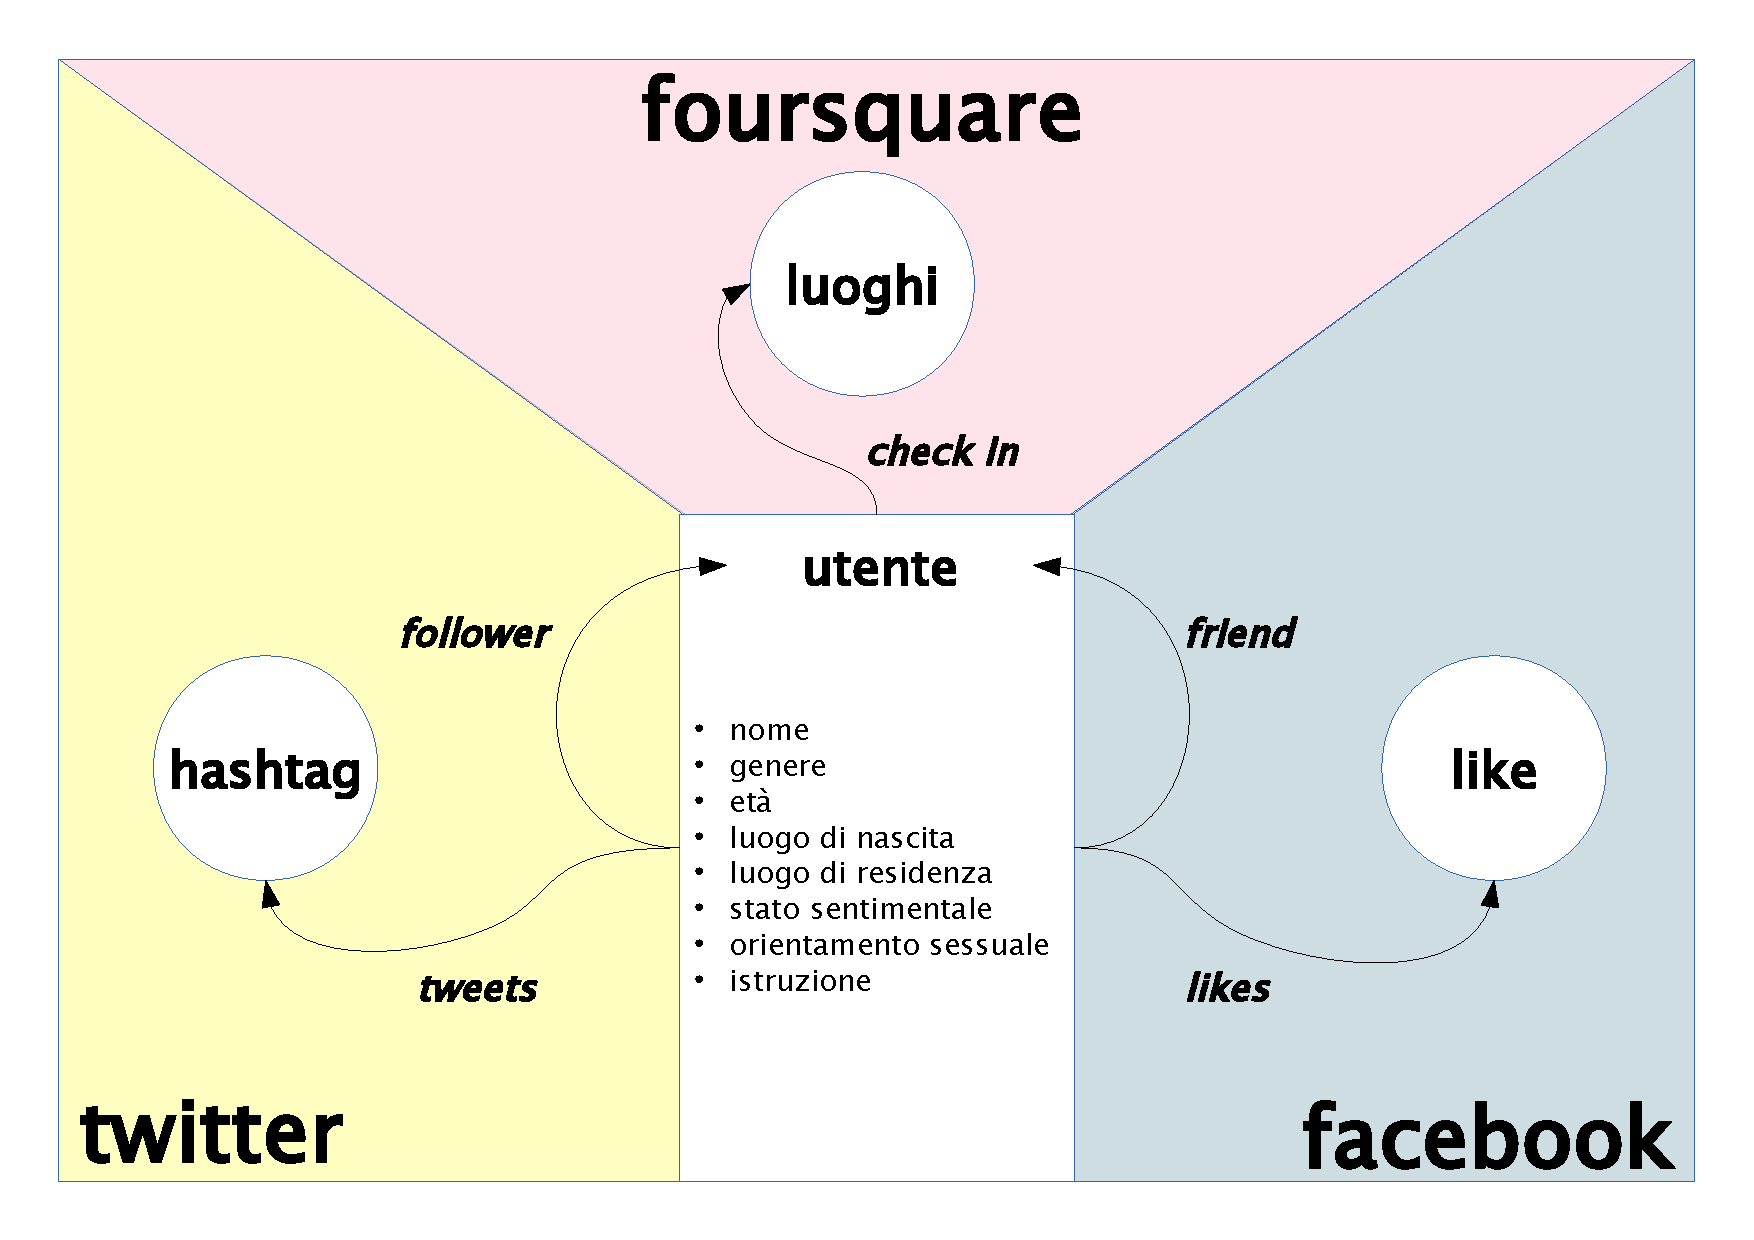
\includegraphics[width=0.95\textwidth]{pictures/modello_dati.pdf}
    \caption{Modello dei dati}
    \label{fig:modello_dati}
\end{figure}
\subsection{Problematiche di integrazione fra le sorgenti}
L'obiettivo finale � definire un modello unico dei dati, come esposto in \autoref{fig:modello_dati}, per integrare tre sorgenti eterogenee.\\
Una evidente differenza fra Twitter e Facebook � la natura e lo scopo delle interazioni fra gli utenti. Facebook � solitamente usato per stare in contatto con persone che si conosce nella vita reale e ritrovare chi si � frequentato nel passato. In particolare, una volta stretta amicizia il rapporto tra due amici � paritario e simmetrico: possono scambiarsi liberamente messaggi ed ogni contenuto pubblicato da una parte viene notificato all'altra. Al contrario, Twitter � principalmente adoperato per comunicare con persone con le quali, pur non frequentandole nella vita reale, si condividono interessi o argomenti di discussione. Questo legame pi� superficiale incide sul grado di omofilia nella rete: individui connessi come \textit{friend} saranno in genere pi� simili di individui connessi come \textit{follower}, tanto pi� se la relazione non � reciproca. Twitter realizza un modello asimmetrico di relazione, in cui la discrepanza tra il numero di persone che ci seguono e quelle che seguiamo determina la reputazione dell'individuo all'interno della comunit�. Nella pratica, l'asimmetria limita i privilegi del \textit{follower} che, ad esempio, non pu� contattare unilateralmente le persone che segue, a meno che non sia stato esplicitamente autorizzato o la relazione sia stata ricambiata. Questa peculiarit� ha sensibili implicazioni sul modello dei dati, giacch� il grafo degli utenti deve adesso contenere archi orientati.\\
Una ulteriore peculiarit� risiede nel confronto tra \textit{like} e \textit{hashtag}. Mentre la relazione tra un utente Facebook e un like � binaria---o l'utente ha espresso il proprio gradimento di un oggetto o non lo ha fatto---nel caso di Twitter un utente pu� non adoperare mai un hashtag o usarlo con frequenza. Anche in questo caso il modello dei dati richiede una estensione, tramite l'introduzione di pesi sugli archi utente-hashtag. A differenza del caso precedente, dove un arco non orientato pu� essere equivalentemente modellato da una coppia di archi orientati, conciliare gli archi privi di peso di Facebook con quelli pesati di Twitter richiede una normalizzazione arbitraria dei pesi. In aggiunta, il significato di un hashtag � tutt'altro che analogo ad un like, poich�, avendo fissato l'argomento, un tweet pu� esprimere tanto apprezzamento quanto avversione, discussione o ``inutile chiacchiera''\footnote{\url{http://web.archive.org/web/20110715062407/www.pearanalytics.com/blog/wp-content/uploads/2010/05/Twitter-Study-August-2009.pdf}}. Per amalgamare semanticamente i tweet ai like sarebbe necessario discriminare i tweet in semplici categorie---\textit{like} e \textit{dislike}---che tuttavia � un problema di elaborazione del linguaggio naturale e clustering in s�. Infine, la vita media di un hashtag � di gran lunga pi� breve rispetto ad un like. In termini assoluti, mentre un like � sostenuto da un contenuto---una pagina o una realt� esterna a Facebook---la creazione di un hashtag richiede al pi� uno sforzo di immaginazione; la controparte della proliferazione degli hashtag � proprio la loro volatilit�. In termini relativi, il carattere episodico e conversevole del tweet richiede tempi di elaborazione ed azione pi� stringenti, in quanto l'associazione e il coinvolgimento dell'utente rispetto ad un hashtag pu� rapidamente consumarsi. In sintesi, l'analisi dei tweet richiede algoritmi tolleranti di una elevatissima dimensionalit�, coerente con l'elaborazione del linguaggio naturale, possibilmente basati su grafi e che garantiscano una bassa complessit� temporale anche a scapito della qualit�.\\
In ultimo, Foursquare � un servizio unico nel suo genere e, contribuendo informazione nuova e non ridondante, non richiede sforzi addizionali di assimilazione nel modello.\\
Una volta definiti i criteri di integrazione, l'ultimo passo sarebbe la \textit{entity resolution} ovvero l'identificazione dei profili che, bench� apparentemente scorrelati e provenienti da sorgenti diverse, appartengono al medesimo individuo reale.\\
La quantit� di dati a disposizione di Neosperience si � rivelata, comunque, molto al di sotto del volume prospettato a regime, sul quale gli algoritmi e le tecniche di data mining avrebbero dovuto essere messe alla prova. Pertanto, il lavoro si � articolato nei seguenti passi:
\begin{itemize}
\item \hyperref[raccolta_dati]{raccolta dei dati}
\item \hyperref[selezione_algoritmi]{selezione degli algoritmi}
\item \hyperref[preparazione_dati]{preparazione dei dati}
\item \hyperref[esecuzione_algoritmi]{esecuzione degli algoritmi}
\item \hyperref[capitolo4]{analisi dei risultati}
\end{itemize}
\section{Raccolta dei dati}
\label{raccolta_dati}
Le \mbox{\textit{Graph API}}\footnote{\url{https://developers.facebook.com/docs/graph-api}} sono lo strumento principale che permette di leggere e scrivere sul grafo sociale di Facebook. Il grafo sociale � una rappresentazione delle informazioni presenti nel social network composto da:
\begin{itemize}
\item \textbf{nodi}: entit� di vario tipo come utenti, foto, eventi, pagine o commenti, etichettati da un identificatore unico
\item \textbf{archi}: connessioni esistenti tra le entit�: relazioni d'amicizia tra utenti, foto in una pagina, commento su certo un evento, etc.
\item \textbf{campi}: attributi delle entit� come il compleanno di un utente o il nome di una pagina.
\end{itemize}
La maggior parte delle richieste fatte con le Graph API necessita di un \textit{access token}, che consente un accesso temporaneo e sicuro alle informazioni di profilo di un utente. In particolare, l'access token deve essere composto con una serie di permessi a seconda di quale attributo si vuole leggere o scrivere: ad esempio, se si � interessati al nome, al genere e agli amici di un certo individuo, esso deve considerare, simultaneamente, i permessi \texttt{user\_about\_me}, \texttt{user\_gender} e \texttt{user\_friends}.\\
Per recuperare queste informazioni � sufficiente una chiamata al metodo \texttt{HTTP GET}:
\begin{lstlisting}[basicstyle=\normalfont\ttfamily\scriptsize,backgroundcolor=\color{background}]
GET https://graph.facebook.com/me?fields=name,gender,friends
\end{lstlisting}
che restituisce il seguente file JSON\footnote{JavaScript Object Notation, \url{http://www.json.org}}:
\begin{lstlisting}[language=json,firstnumber=1]
{
  "name": "Nicola P.", 
  "gender": "male",
  "friends": {
    "data": [
      { "name": "Linda",  "id": "987654321" },
      {	"name": "Matteo", "id": "123123123" }
    ]
   }
}
\end{lstlisting}

\subsection{Applicazione per la raccolta dei dati}
Mediante l'SDK per PHP\footnote{\url{https://developers.facebook.com/docs/reference/php/4.0.0}} abbiamo creato un'applicazione che ha ci permesso di recuperare da un utente le seguenti tipologie d'informazione: \textit{profilo} (data di nascita, genere, orientamento sessuale, stato sentimentale, citt� natale, citt� di residenza  e istruzione), \textit{like} (tutte le pagine su cui si � indicato \textit{like}) e \textit{amici} (profilo e like degli amici).\\
L'applicazione � stata utilizzata da 87 utenti (che abbiamo indicato con il termine \textit{DAU} o \textit{Direct User Application}) ottenendo, in totale, circa 25 mila profili Facebook in formato JSON.\\
Il passo successivo � stato quello di unificare tutti i profili in un unico file GML\footnote{Il formato GML (Graph Modelling Language) permette la rappresentazione dettagliata di un grafo con attributi}. Dal file JSON di ogni DAU sono stati recuperati gli identificatori degli amici e quindi i file JSON ad essi corrispondenti: in questa maniera � stato possibile costruire la rete personale del DAU (o \textit{ego-network}) arricchita dalle informazioni di profilo e dai like di ogni nodo. La composizione incrementale di queste reti ha portato alla creazione del grafo finale.

%\subsubsection{Pulizia preliminare dei nodi}
%Il grafo � stato ripulito da un insieme di nodi problematici sotto due aspetti. Un utente, infatti, viene escluso se: (1) il numero di attributi di profilo mancanti � maggiore della met�, e (2) se presenta un valore mancante per un certo attributo e la percentuale dei suoi vicini che, per lo stesso attributo hanno valore mancante, � maggiore del cinquanta percento. Il primo punto � di immediata comprensione, il secondo � giustificato dal fatto che l'inferenza di un certo attributo di un utente � basata sui valori che quell'attributo possiede nei vicini dell'utente stesso: se pi� della met� dei vicini hanno un valore mancante allora � lecito pensare che l'inferenza pu� addurre risultati molto approssimativi.

\subsection{Creazione dei sottografi}
\label{sampler}
Come gi� accennato in precedenza, abbiamo sviluppato uno strumento\footnote{Il linguaggio utilizzato per la creazione di questo tool � Gremlin (\url{https://github.com/tinkerpop/gremlin/wiki}) che permette di comporre query su grafi} per il campionamento di grafi che, da un lato, riuscisse a creare sottografi significativi dal punto di vista topologico e degli attributi; dall'altro, che presentasse una forte componente casuale per modellare la variet� dei dati in input che potrebbero essere utilizzati successivamente.\\
Il procedimento adottato � il seguente:
\begin{enumerate}
\item si sceglie casualmente un DAU $ X $ non ancora considerato
\item si recuperano i vicini di $ X $ non ancora considerati
\item con un certa probabilit� $ p $ si sceglie un vicino $ Y $ di $ X $; altrimenti si torna a 1, scegliendo casualmente un altro DAU
\item se si � scelto il vicino $ Y $ di $ X $ si scala la probabilit� $ p $ di un fattore $ s < 1 $, si pone $ X = Y $ e si torna ad 1.
\end{enumerate}
Questo procedimento viene ripetuto fino a quando non si raggiunge una certa percentuale $ \pi $ di utenti considerati.\\
Un DAU � un nodo ricco di informazioni, quindi � fondamentale che esso venga scelto come punto di partenza del campionamento. Con una probabilit� che scala progressivamente, si considerano i suoi vicini e i vicini dei vicini, costruendo cos� una rete collegata al DAU iniziale. Successivamente, scegliendo un nuovo DAU (cio� partendo di nuovo dal punto 1) si ha la possibilit� di costruire una rete ulteriore che, a seconda dei casi, sar� collegata o meno alla prima. Questo procedimento iterativo porta, infine, alla selezione di un insieme di nodi su cui � possibile indurre il grafo campionato.\\
Variando i tre parametri ($ p $, $ s $ e $ \pi $) siamo stati in grado di generare una vasta gamma di sottografi che presentano caratteristiche topologiche e di attributi molto variegate. 

\section{Selezione degli algoritmi}
\label{selezione_algoritmi}
In considerazione della variet� dei dataset su cui avremmo operato, abbiamo selezionato una vasta gamma di algoritmi, cercando di differenziarli per modello dei dati utilizzato, tecnica di clustering (\ref{sec:classificazione_algoritmi}), approccio alla dimensionalit� (\ref{subsec:subspace_clustering}) e prestazioni.\\
Limitatamente al modello dei dati, gli algoritmi possono essere raggruppati in tre categorie:
\begin{itemize}
\item clustering su attributi: NetClus \cite{netclus}, MOC \cite{moc}, LAC \cite{lac}, ORCLUS \cite{orclus}
\item clustering su grafo: Fast Unfolding \cite{blondel2008fuc}
\item clustering su attributi e grafo: LatentNet \cite{handcock07}, CESNA \cite{cesna}, Inc-Cluster \cite{inc_cluster}, DB-CSC \cite{db_csc}, BAGC \cite{bagc}
\end{itemize}
\subsection{Descrizione degli algoritmi}
Di seguito mostreremo, per il lettore interessato, la descrizione teorica dei vari algoritmi a nostra disposizione.
\begin{description}
\item[NetClus] � un algoritmo per il clustering di reti composte da entit� eterogenee e conformazione a stella (\textit{star network schema}). In assenza di connessioni tra utenti, il modello dei dati descritto in \autoref{fig:modello_dati} riflette esattamente questo scenario: al centro della stella vi � l'utente, da cui scaturiscono archi verso gli attributi di profilo, like, hashtag e check-in, ognuno dei quali forma un nuovo tipo di entit�. Il pregio di NetClus � che non si limita ad attribuire una etichetta di cluster a ciascun utente, ma produce un ordinamento dei valori di ciascuna entit� in ognuno dei cluster ottenuti, semplificando notevolmente l'interpretazione dei risultati.
%Ad esempio, per ogni cluster sarebbero evidenziati i valori di et�, luogo di nascita, grado di istruzione, like, check-in\dots pi� rappresentativi per la popolazione raccolta nel cluster.
In secondo luogo, l'approccio di NetClus riduce fortemente la dimensionalit� del problema rispetto agli altri algoritmi su attributi, dove ogni nuovo like o hashtag aggiunge una dimensione al dataset. Un ultimo punto di forza � che non richiede la definizione di una misura di similarit�, ma costruisce un modello probabilistico generativo sotto l'ipotesi che la rete esibisca assortativit� e \textit{preferential attachment}, come nel caso delle reti sociali. Dato il numero di cluster, l'idea generale di NetClus si compone dei seguenti passi: generare una partizione iniziale degli oggetti ed indurre i \textit{net-cluster} $\{C_{k}^{0}\}_{k=1}^{K}$ dalla rete originale sulla base di queste partizioni; costruire, per ciascun net-cluster, un modello probabilistico generativo $\{P(x|C_{k}^{t})\}_{k=1}^{K}$; quindi calcolare la probabilit� a posteriori $P(C_{k}^{t}|x)$ per ciascun oggetto e ricalcolare l'assegnamento degli oggetti ai cluster. I due passi precedenti sono reiterati finch� i cluster non raggiungono una condizione stazionaria. Al termine, dalla probabilit� a posteriori si ottiene un ordinamento degli oggetti all'interno dei cluster di appartenenza. L'algoritmo ha complessit� lineare nel numero di archi, ovvero per reti sparse � approssimativamente lineare nel numero di nodi.

\item[MOC] � un algoritmo probabilistico generativo per l'identificazione di cluster non disgiunti o \textit{overlapping}. L'algoritmo generalizza e semplifica un precedente studio sul clustering sovrapposto di espressioni genetiche \cite{SegalBK03}; con una scelta oculata del modello di probabilit� e definizione di distanza---la famiglia esponenziale e la divergenza di Bregman rispettivamente---gli autori sostengono di poter applicare la tecnica a dati sparsi e con numerose dimensioni, laddove il modello gaussiano e la distanza euclidea, usati pi� comunemente, sono noti offrire scarsi risultati. A testimonianza della formulazione originale, i dati o matrice di espressione $X$ sono modellati come la manifestazione di due fattori, l'appartenenza $M$ e l'attivazione $A$. L'appartenenza descrive quanto i cluster nascosti nei dati si manifestano in ciascun individuo; dato che il modello � \textit{overlapping}, ogni individuo pu� appartenere simultaneamente a pi� cluster. L'attivazione indica il peso di ciascuna dimensione dei dati in ognuno dei cluster, ossia quali caratteristiche di un individuo sono determinate pi� significativamente dall'appartenenza al cluster. I dati sono quindi ricostruiti come il prodotto $X'=M \times A$ tra la matrice di appartenenza e la matrice di attivazione. Seguendo questa intuizione, l'algoritmo costruisce una stima iterativa di $M$ e $A$. Il vettore di appartenenza $M_i$ di ciascun individuo � ottenuto con un approccio \textit{greedy}, volto a minimizzare la distanza tra l'individuo e la sua approssimazione $M_i \times A$: fissata la matrice di attivazione $A$, MOC `accende' con ogni iterazione un nuovo cluster, fino a quando per nessuna scelta � possibile ridurre ulteriormente la funzione obiettivo. La complessit� temporale di questa fase � $O(k^3)$ nel numero di cluster $k$. La matrice di attivazione pu� essere costruita dalla minimizzazione della medesima funzione obiettivo, fissata $M$; seppure sia definita una diversa formula per ogni modello nella famiglia esponenziale e relativa divergenza, la complessit� temporale di questa fase pu� essere stimata in $O(d^3)$.
\item[LAC] � un algoritmo \textit{centroid-based} di \textit{subspace clustering}. Come discusso in \ref{subsec:metodi_partitivi}, le prestazioni degli algoritmi basati sulla distanza euclidea degradano rapidamente al crescere del numero di dimensioni. Per ovviare a questo noto limite, LAC trasforma lo spazio in cui ciascun cluster � immerso, associando ad ogni cluster un vettore di pesi affinch� maggiore importanza sia conferita alle dimensioni lungo le quali c'� aggregazione dei punti, all'interno del cluster. I pesi indicano quindi il grado di partecipazione di ciascun attributo al cluster; se i punti sono fortemente raggruppati rispetto a quell'attributo, il peso sar� alto, e basso altrimenti. Questi coefficienti sono appresi iterativamente con la ottimizzazione della somma degli errori quadrati (SSE), ovvero, per ciascun cluster, le distanze tra il centroide di riferimento e tutti i punti appartenenti al cluster. In assenza di contromisure, tutto il peso sarebbe concentrato sulla dimensione a minima varianza e l'algoritmo scoprirebbe unicamente cluster monodimensionali; per controllare la dimensione dello sottospazio in cui i cluster sono valutati, l'utente deve fissare un termine di penalit� che � inserito nella funzione obiettivo. Sebbene l'esistenza di parametri astratti come questo sia un aspetto in genere indesiderabile, gli autori hanno definito una metodologia \textit{ensemble} per la determinazione del valore ottimo attraverso esecuzioni multiple della procedura di clustering. Ogni iterazione dell'algoritmo ha complessit� $O(kDN)$, dove $k$ � il numero di cluster, $N$ il numero di elementi del dataset e $D$ il numero di dimensioni; il tempo di esecuzione � quindi governato dalla rapidit� con cui l'algoritmo converge ad una soluzione.
\item[ORCLUS] � un algoritmo di clustering proiettato (\textit{projected clustering}) basato su \textit{K}-medoids. Dati due parametri specificati dall'utente, il numero di gruppi e il numero di dimensioni dei gruppi, ORCLUS identifica un insieme di cluster arbitrariamente allineati---non solo paralleli agli assi, ma ottenuti dalla combinazione lineare delle dimensioni originali---ciascuno in un sottospazio della dimensione specificata. ORCLUS � molto simile all'algoritmo k-means, tranne per il fatto che, invece di misurare le distanze nello spazio completo, queste sono calcolate nei sottospazi di ciascun cluster. Preliminarmente, ORCLUS sceglie casualmente dei `semi' o potenziali medoidi. L'algoritmo richiede quindi un processo iterativo: in ogni iterazione ciascun cluster � progressivamente raffinato, rimuovendo le dimensioni prive di aggregazione e riducendo il numero di cluster dall'accorpamento di quelli pi� simili. I sottospazi sono formati tramite PCA, ovvero calcolando la matrice di covarianza per ciascun cluster e selezionando gli autovettori con la minore diffusione nel sottospazio del cluster, ovvero quelli associati agli autovalori pi� piccoli. Quando due cluster sono vicini e hanno simili direzioni degli autovettori sono fusi assieme. A chiusura di ogni iterazione � eseguita la fase di assegnamento: ogni punto � associato al seme pi� vicino e i semi sono ricalcolati come i centroidi dei cluster appena formati. L'algoritmo � computazionalmente intensivo $O(d^3)$ nella dimensione dei dati, in conseguenza del calcolo della matrice di covarianza e degli autovettori di ciascun cluster. Oltretutto, richiede la specificazione non solo del numero di cluster ma anche della dimensione del sottospazio in cui ciascun cluster � costruito, un parametro difficile da stimare correttamente a priori.
\item[LatentNet] � un algoritmo di clustering probabilistico, basato su un modello generativo. Partendo da un grafo di relazioni binarie, il modello assume che ogni nodo possieda una posizione non osservabile in uno spazio sociale \mbox{\textit{d}-dimensionale}, euclideo e latente. Con questa premessa, la presenza o l'assenza di una connessione tra due individui � indipendente da ogni altra informazione, se sono note le posizioni dei due individui nello spazio sociale. Questo modello esprime in maniera innata tanto la transitivit� quanto l'omofilia negli attributi osservati. Per introdurre la propriet� di clustering, si assume che le posizioni nello spazio latente siano estratte da un modello misto (\textit{mixture model}) di distribuzioni Gaussiane multivariate: ogni distribuzione � caratterizzata da una propria media e varianza, e rappresenta un diverso gruppo di individui o cluster. Per la stima delle posizioni nello spazio latente, gli autori propongono due metodi. Il primo � un metodo in due fasi: inizialmente calcola la stima a massima verosimiglianza del modello dello spazio latente---che spiega la transitivit� e l'omofilia---e determina le posizioni degli attori nello spazio sociale; la seconda fase stima i parametri del modello misto, basandosi sulle posizioni nello spazio latente ottenute nella prima fase. Il secondo metodo � pienamente Bayesiano e usa \textit{MCMC sampling}: il vantaggio � che stima simultaneamente le posizioni latenti e il modello di clustering, ma � computazionalmente pi� esigente.

\item [Fast Unfolding] � un algoritmo euristico per il clustering di grafi basato sull'ottimizzazione della modularit�. Il metodo � diviso in due fasi che vengono ripetute ciclicamente. All'inizio, si considerano tante comunit� quanti sono i nodi della rete. Successivamente, per ogni nodo $ i $ si considerano i suoi vicini $ j $ e si valuta il guadagno della modularit� che si avrebbe se si spostasse il nodo dalla sua comunit� alla comunit� di un nodo $ j $: il nodo $ i $ viene effettivamente spostato in quella comunit� che genera il massimo guadagno positivo. Se ci� non � possibile il nodo resta nella sua comunit�. Questa prima fase viene ripetuta sequenzialmente per ogni nodo, finch� non � possibile nessun ulteriore miglioramento. La seconda fase consiste nel costruire un nuovo grafo i cui nodi sono le comunit� trovate durante la prima fase: gli archi di ogni nuovo \virgolette{nodo-comunit�} sono l'unione degli archi dei nodi atomici che lo compongono. Al termine di questa seconda fase si pu� applicare di nuovo la prima, in un processo iterativo che termina quando non � pi� possibile spostare un nodo in una comunit� diversa ed avere un guadagno positivo della modularit�.
\item [Inc-Cluster] � un algoritmo di clustering per grafi con attributi. Per ogni coppia attributo-valore $ (a, v) $ del dataset viene aggiunto, nel grafo originale, un nodo $ n_{a,v} $ che sar� collegato a tutti i vertici che presentano il valore $ v $ per l'attributo $ a $. In questo modo viene creato un grafo \textit{aumentato} su cui � possibile definire una funzione di distanza (la \textit{random walk distance}) che tenga conto sia dell'informazione topologica sia del valore degli attributi dei nodi: infatti la funzione di distanza considera \textit{simili} due individui se ci sono numerosi percorsi che li collegano. Poich� nel grafo aumentato i percorsi tra i nodi sono possibili anche grazie alla presenza degli attributi che condividono e non solo per le relazioni d'amicizia, allora � facile immaginare in che senso la funzione distanza riesce a tener conto, contemporaneamente, della ego-network dei due nodi e della similarit� tra i loro attributi. L'algoritmo utilizza una tecnica molto simile a quella del K-Medoids iterando l'assegnamento di un nodo ai vari \virgolette{centroidi} fino a alla convergenza della funzione obiettivo. Purtroppo il calcolo della similarit� degli utenti � computazionalmente inefficiente, $ O(n^{2.807}) $ con $ n $ numero di nodi del grafo. Infine, Inc-Cluster richiede di specificare non solo il numero di cluster, ma anche probabilit� di \textit{restart} e la lunghezza massima del percorsi nelle random walk.
\item [DB-CSC] � un algoritmo di clustering per grafi con attributi, basato sul concetto di densit�: esso individua, infatti, regioni dense sia nel grafo che nello spazio degli attributi. In particolare, per ogni nodo $ v $ vengono definiti la $ \epsilon \mdash neighborhood $, cio� l'insieme dei vicini che distano al massimo $ \epsilon $ da $ v $, e la $ k \mdash neighborhood $ cio� l'insieme dei vicini che raggiungono $ v $ in  $ k $ passi al massimo. L'intersezione tra $ \epsilon \mdash neighborhood $ e $ k \mdash neighborhood $ rappresenta il \textit{vicinato locale} di un nodo. L'algoritmo definisce un cluster come un insieme di vertici $ O $ tali per cui, (1) ogni vertice $ v \in O $ ha un vicinato locale molto numeroso (cio� la cui cardinalit� � maggiore di $ minPts $, definito dall'utente) e (2) per ogni coppia di punti in $ O $ esiste sempre un cammino che li collega.
Successivamente, viene costruito un grafo \textit{arricchito} in questa maniera: se due nodi del grafo originale hanno attributi simili e sono connessi da $ k $ archi al massimo (ovvero, se appartengono allo stesso vicinato locale) allora verranno collegati nel grafo arricchito. Dal grafo arricchito si calcolano tutti i $ (minPts-1) \mdash core$\footnote{Dato un grafo $ G $, un $ c \mdash core $  � un sottografo di G connesso e massimale in cui tutti i vertici hanno un grado maggiore o uguale a $ c $}, che rappresentano delle comunit� potenziali: se il grafo arricchito contiene un unico $ (minPts-1) \mdash core $ che copre ogni nodo allora esso � un cluster valido secondo la definizione sopracitata; altrimenti bisogna ripetere questa considerazione per ognuno dei $ (minPts-1) \mdash core $ presenti nel grafo arricchito. Ricorsivamente si individuano i grafi arricchiti indotti dai nodi di ogni $ (minPts-1) \mdash core $ e su questi si calcolano, ancora una volta, i $ (minPts-1) \mdash core $: se ogni grafo arricchito � composto da un singolo $ (minPts-1) \mdash core $ che copre tutti i suoi nodi allora esso � una comunit�.
Questa procedura viene, infine, generalizzata per individuare i cluster in ogni sottospazio degli attributi originali.

\item[CESNA] � un algoritmo probabilistico generativo per l'identificazione di comunit� non disgiunte (\textit{overlapping}) su grafi con attributi. Per la costruzione del modello probabilistico vengono individuate due variabili osservabili, il grafo $ G $ e l'insieme di attributi $ X $, e una variabile latente da inferire, la funzione di \textit{membership} $ F $ che indica, per ogni nodo, qual � il grado di appartenenza ad una certa comunit�. A questo punto � possibile definire due sotto-modelli generativi. Il \textit{modello degli archi della rete}, stabilisce qual � la probabilit� che due nodi sono collegati tra loro in funzione della loro membership: essi avranno un'alta probabilit� di essere collegati se condividono un elevato numero di comunit�.\\
CESNA � l'unico algoritmo, tra quelli selezionati, che supporta i valori mancanti (\textit{missing value}): per ogni coppia attributo-valore $ (a, v) $ si crea una \textit{propriet�} $ k $ che viene associata a tutti e soli gli utenti che presentano il valore $ v $ per l'attributo $ a $. Quindi, il \textit{modello degli attributi dei nodi}, stabilisce qual � la probabilit� che un certo nodo $ u $  esponga la propriet� $ k $. Successivamente, si introduce un'altra variabile latente (anch'essa da inferire): il peso $ W $ di una propriet� all'interno di un certo cluster. Se il nodo $ x $ partecipa a un certo numero di cluster per cui il peso di $ k $ � alto, allora � molto probabile che $ x $ possieda $ k $. Questo modello fa in modo che i nodi che appartengono alla stessa comunit� condividono, probabilmente, le stesse propriet�.\\
Infine, viene costruito il modello \textit{combinato} che, in estrema sintesi, rappresenta la probabilit� di avere un certo grafo $ G $ e un insieme di attributi $ X $ conoscendo la funzione di membership $ F $ e il set di pesi $ W $: $ P(G, X | F, W) $. Si suppone ora che questo modello generi i dati in input all'algoritmo e quindi, per spiegarli e giustificarli al meglio, si deve determinare la coppia $ \hat{F} $ e $ \hat{W} $ che massimizza la verosimiglianza $ log P(G,X | F,W) $. Se il grado di appartenenza di un nodo ad una certa comunit� supera una soglia $ \delta $ allora il nodo appartiene a quella comunit�; se un nodo presenta, per tutte le comunit�, una membership minore di $ \delta $ allora viene considerato un outlier.\\
La complessit� computazionale � lineare nel numero dei nodi $N$, degli archi $E$ e nel numero di attributi $K$: $ O (E + NK) $.

\item[BAGC] � un algoritmo probabilistico generativo per il clustering di grafi con attributi. Idealmente, BAGC attribuisce ad ogni possibile clustering sui dati una probabilit�, cosicch� il miglior clustering � semplicemente quello pi� verosimile, che massimizza la probabilit�. Nonostante la semplicit� concettuale di tale approccio, esplorare interamente lo spazio dei clustering possibili � impraticabile, e l'algoritmo propone una soluzione approssimata. Il primo passo � individuare una distribuzione parametrica che approssimi la probabilit� congiunta tra il grafo considerato e i possibili clustering, modellando separatamente l'etichetta di cluster, gli attributi e gli archi per ciascun vertice. Avendo espresso il clustering come un problema di ottimizzazione---trovare il massimo a posteriori della divisione in cluster condizionatamente al grafo e agli attributi dati---devono essere caratterizzate le condizioni di stazionariet�, per potersi arrestare nella ricerca iterativa del valore ottimo. La soluzione approssimata � quindi raggiunta con un metodo variazionale.

\item[ROCK] � un tecnica gerarchica (bottom-up) per il clustering overlapping su attributi categorici. Per raggruppare gli oggetti del dataset, l'algoritmo non utilizza una semplice funzione di similarit� (come l'indice Jaccard) poich� questa pu� rivelarsi poco conveniente in molte situazioni. Si pensi, in maniera intuitiva, al caso in cui due punti sono \textit{distanti} tra loro ma presentano un insieme di \virgolette{vicini} molto simili: una misura standard non considerer� quest'ultimo aspetto e un algoritmo gerarchico non decider� mai di raggruppare insieme i due punti. Per ovviare a questo problema, gli autori propongono una misura \textit{globale} che consideri non solo i punti in s� ma anche la distribuzione del loro \textit{vicinato}. Si definisce, quindi, il numero di \textit{link} tra due oggetti come il numero di vicini che hanno in comune;\footnote{In generale il numero di link � calcolato su due insiemi di punti ed indica, semplicemente, il numero di vicini comuni a tutti gli elementi degli insiemi} inoltre, due oggetti sono detti \textit{vicini} se la loro distanza non supera una certa soglia definita dall'utente. Come ogni algoritmo gerarchico bottom-up, ROCK inizia col considerare tanti cluster quanti sono gli oggetti del dataset per poi agglomerare, iterativamente, le coppie di cluster che massimizzano una misura di \textit{bont�} proporzionale al numero di link. La complessit� computazione � $ O(m_{a}n^{2}) $ dove $ m_{a} $ � il numero medio dei vicini di un punto.

\end{description}
\section{Preparazione dei dati}
\label{preparazione_dati}
I profili utente si sono rivelati spesso inaccurati, disseminati di dati inverosimili e omissioni. Purtroppo, la cattiva qualit� � una caratteristica dei dati reali, in cui il rumore, le imprecisioni della rilevazione e l'informazione mancante pregiudicano il successo del data mining. Per questo motivo, la qualit� del clustering dipende tanto dalla adeguatezza della tecnica impiegata quanto dall'abilit� dell'analista di preparare i dati per l'analisi.
\subsection{Rimozione degli outlier}
%Un outlier � un individuo che devia significativamente dal resto della popolazione; contrariamente al rumore, che esprime le naturali differenze tra le persone, l'anomalia � generata da un meccanismo e risponde a regole radicalmente diversi da quelle valide per gli altri individui.
La ricerca degli outlier � spesso un fine in s�---come l'identificazione delle intrusioni informatiche e delle frodi bancarie---ma in questo lavoro siamo interessati unicamente a prevenire le distorsioni numeriche che un outlier produce. Identificare un individuo atipico nel contesto delle reti sociali non � semplice, poich� la numerosit� delle dimensioni rende insignificanti la distanza e la densit�, che sono alla base delle procedure canoniche per l'identificazione delle anomalie (\autoref{subsubsec:outlier}). Non � neppure sufficiente basarsi sulla topologia del grafo delle amicizie, e dichiarare anomali gli individui debolmente connessi alla popolazione. Poich� abbiamo una visione parziale della rete, le connessioni che potrebbero contribuire ad integrare un individuo sono spesso inosservate, e questo limite si accentua ulteriormente nei campioni estratti dal dataset completo. Infine, anche i like possono essere fuorvianti, poich� risultano empiricamente molto sparsi: come discuteremo in \autoref{subsubsec:discretizzazione}, la popolarit� media di un singolo like � estremamente bassa, meno di 5 utenti su oltre 25000. Ci siamo pertanto limitati a ricercare gli utenti che avessero un profilo platealmente abnorme. A tal fine, abbiamo misurato tramite la distanza di Mahalanobis la dissimilarit� di ciascun individuo rispetto alla media della popolazione, trasformando cos� un problema multivariato---in considerazione del numero di attributi di ciascun individuo---in uno univariato. A questo punto � possibile applicare al vettore di distanze una tecnica arbitraria di identificazione degli outlier: test Chi-quadro, gaussiano, Local-Outlier-Factor etc. Partendo da questa selezione, abbiamo poi ispezionato individualmente i candidati e rimosso quelli che, a nostro giudizio, fossero effettivamente incompatibili con la popolazione.

\subsection{Inferire i valori mancanti}
A ciascun utente sono associati due tipi di propriet�: il profilo e i like. I like sono ovviamente variabili da un individuo all'altro, n� ha senso trattare l'assenza di un \textit{mi piace} su un certo contenuto come valore mancante. In generale, parliamo quindi di valori mancanti solo per i dati di profilo, dove sono raccolte le informazioni biografiche dell'utente. Una ulteriore ragione per dare maggior peso all'assenza di informazione di profilo rispetto ai like � il ruolo che questi dati rivestiranno nell'analisi. Mentre i like sono fondamentali per produrre il clustering, gli attributi di profilo sono decisivi per interpretarlo. Una volta individuati i cluster, attraverso i like siamo in grado di capire quali interessi accomunano le persone; tuttavia, assumendo di non avere altre fonti di informazione, senza i dati del profilo non � possibile caratterizzare questi gruppi e descrivere le persone che ne fanno parte con le variabili della segmentazione tradizionale.\\
Tra gli algoritmi che abbiamo selezionato, solo CESNA \cite{cesna} tollera i valori mancanti; per tutti gli altri � stato necessario produrre una versione completa dei dati. In questa fase abbiamo fatto ricorso a tre soluzioni: rimuovere l'individuo con valori mancanti (la riga del dataset), rimuovere integralmente l'attributo (la colonna del dataset) o inferire il valore laddove assente. La prima soluzione � consigliabile quando l'individuo � cos� povero di informazione da non produrre alcun beneficio all'analisi. La seconda soluzione, eliminare integralmente una dimensione, � necessaria quando l'attributo � assente per una significativa porzione della popolazione: in questo scenario, rimuovere gli individui privi dell'attributo sarebbe un spreco di dati e non � nemmeno disponibile sufficiente informazione reale per inferire i valori mancanti. Dalle statistiche in \autoref{table:missing_values} si nota che gli attributi \textit{orientamento sessuale} e \textit{stato sentimentale} sono specificati da una estrema minoranza di utenti e sono stati pertanto rimossi dal dataset.
\begin{table}[h]
\resizebox{0.9\textwidth}{!}{\begin{minipage}{\textwidth}
\centering
\begin{tabular}{| c | c | c | c | c | c | c | }
\multicolumn{1}{c}{genere}
 &  \multicolumn{1}{c}{et�}
 & \multicolumn{1}{c}{\specialcell[t]{luogo di\\nascita}}
 & \multicolumn{1}{c}{\specialcell[t]{luogo di\\residenza}}
 & \multicolumn{1}{c}{educazione}
 & \multicolumn{1}{c}{\specialcell[t]{orientamento\\sessuale}}
 & \multicolumn{1}{c}{\specialcell[t]{stato\\sentimentale}}
 \tabularnewline
\cline{1-7}
0.78\% & 32.53\% & 28.02\% & 23.64\% & 24.29\% & 99.13\% & 99.84\%\tabularnewline
\cline{1-7}
\end{tabular}
\caption{Distribuzione dei valori mancanti per attributo}
\label{table:missing_values}
\end{minipage} }
\end{table}\\
In ultimo, gli attributi non specificati possono essere dedotti tramite imputazione, ma la procedura da adottare dipende dalla natura del valore mancante. Alla radice dell'informazione incompleta vi sono cause disparate: un profilo sostanzialmente inattivo, l'irrilevanza dell'informazione per l'utente o semplicemente il desiderio di privacy. Richiamando la terminologia introdotta in \autoref{subsec:missing_value}, inattivit� e irrilevanza ricadono nella tipologia MCAR, in quanto non vi � alcuna connessione tra il valore dell'attributo mancante e il fatto che non sia stato inserito. La riservatezza invece � generalmente MNAR, poich� dobbiamo conservativamente assumere che il non pubblicare una informazione possa dipendere dal valore dell'attributo per l'utente considerato. I valori mancanti nel nostro dataset sono quindi anche MNAR, e per essi non esiste una procedura univoca di inferenza. Abbiamo deciso pertanto di applicare una tecnica di imputazione ad hoc che faccia leva sull'omofilia nella rete, cio� sul fatto che gli amici di un individuo sono naturalmente selezionati tra i pi� simili ad esso all'interno della popolazione. Per ciascun individuo con valori mancanti, abbiamo considerato gli utenti a cui � connesso nel grafo delle amicizie e stimato da questi il valore dell'attributo mancante. A questo punto, la stima pu� avvenire con uno dei metodi definiti in letteratura: media, hot-deck, regressione etc. Tuttavia, quando un individuo non ha un vicinato sufficientemente ampio, o i vicini a loro volta non possiedono l'attributo mancante nel soggetto, l'imputazione non � affidabile. Pertanto, abbiamo deciso di escludere dal dataset un utente se: (1) il numero di attributi di profilo mancanti � maggiore della met�, e (2) se presenta un valore mancante per un certo attributo che, a sua volta, non � specificato da oltre la met� dei suoi vicini. Con le due fasi di rimozione dei dati impuri, la dimensione del dataset � drasticamente calata; abbiamo quantificato la perdita di informazione in \autoref{table:cleaned_dataset_statistics}.
\begin{table}[h]
\small
\centering
\begin{tabular}{l | c | c | c |}
 \multicolumn{1}{c}{} 
 & \multicolumn{1}{c}{nodi}
 & \multicolumn{1}{c}{archi \textit{friend}}
 & \multicolumn{1}{c}{archi \textit{like}}
 \tabularnewline
\cline{2-4}
originale (con MV) & 25853 & 975\hspace{2pt}382 & 4\hspace{2pt}391\hspace{2pt}494 \tabularnewline
\cline{2-4}
completo (senza MV) & 16336 & 710\hspace{2pt}711 & 3\hspace{2pt}131\hspace{2pt}019 \tabularnewline
\cline{1-4}
decremento assoluto & 9517 & 264\hspace{2pt}671 & 1\hspace{2pt}260\hspace{2pt}475 \tabularnewline
\cline{2-4}
decremento percentuale & 36.81\% & 27.14\% & 28.7\% \tabularnewline
\cline{2-4}
\end{tabular}
\caption{Perdita di informazione durante l'imputazione dei valori mancanti (MV)}
\label{table:cleaned_dataset_statistics}
\end{table}\\
%Missingness by attribute
%interested_in 0.9913379
%gender 0.007874636
%hometown 0.280652
%location 0.2375384
%birthday 0.3262855
%relationship_status 0.9983857
%education 0.2437594
%missingness for education
%HS			College		GR Sc		
%0.3231751 	0.4175526 	0.9296795
%True missing
%HS			College		GR Sc
%0.0794157	0.01204819	0
Si noti che anche la trasformazione degli attributi pu� produrre valori mancanti: nel passare dai nomi dei luoghi alle coordinate geografiche, non � stato talvolta possibile identificare citt� e paesi inseriti dagli utenti, per i quali si � dovuto inferire un valore categorico riconoscibile e convertire quest'ultimo.

\subsection{Selezione degli attributi}
Come gi� anticipato nei paragrafi precedenti (\autoref{data_prepro}), le tecniche di feature selection portano dei vantaggi immediati alla cluster analysis: oltre a velocizzare gli algoritmi di mining, a ridurre la dimensione del dataset e a facilitare la presentazione dei risultati, migliorano significativamente la qualit� e la granularit� del clustering. Infatti, la suddivisione dei dati in gruppi omogenei � molto pi� semplice e nitida in uno spazio con poche dimensioni; inoltre, di frequente, i cluster emergono solamente in un sottoinsieme di attributi restando \virgolette{nascosti} in uno spazio ad elevata dimensionalit� (ad esempio, un gruppo di individui potrebbe essere simile per et�, genere e luogo di nascita ma non per religione e citt� di residenza).\\
In questo lavoro abbiamo utilizzato il tool \texttt{FSFS}\footnote{Feature Selection using Feature Similarity, \url{http://cse.iitkgp.ac.in/~pabitra/paper/fsfs.tar.gz}} che permette di identificare gli attributi pi� significativi all'interno di un dataset in input. � una tecnica non supervisionata che si basa sul concetto di similarit� tra le feature: queste, infatti, vengono raggruppate in vari cluster omogenei per poi selezionare, da ogni cluster, l'attributo pi� significativo. L'algoritmo richiede all'utente di specificare il numero di propriet� $ h $ da rimuovere: � necessario, quindi, condurre degli esperimenti per la regolazione di questo parametro. Tramite la definizione di \textit{entropia di rappresentazione} \cite{Mitra2002} � possibile capire quando un certo sottoinsieme di feature � indicativo o meno: l'entropia di rappresentazione assume valori bassi quando la maggior parte dell'informazione significativa di un dataset � contenuta lungo poche dimensioni, mentre assume valori alti quando l'informazione � equamente distribuita fra tutte le feature. Quindi, studiando l'andamento dell'entropia di rappresentazione del dataset al variare del numero di attributi selezionati, � possibile individuare il miglior valore di $ h $.

\subsection{Trasformazione dei dati}
Come anticipato in \autoref{sec:contesto}, ciascun algoritmo richiede un preciso formato degli input per poter essere applicabile, e i dati, quando non soddisfano tale formulazione, devono essere convertiti. Una frequente ragione di incompatibilit� fra dati e tecniche di clustering � il tipo degli attributi---numerico o categorico---ed il nostro grafo li contiene entrambi. Anche per questo motivo, si � reso necessario scrivere dei convertitori che eseguono la trasformazione del grafo nella formulazione specifica di ciascun algoritmo. Limitatamente al tipo di dato supportato, LAC, MOC e ORCLUS sono numerici, mentre NetClus, LatentNet, CESNA, BAGC e ROCK sono categorici.
\subsubsection{Conversione numerica dei like}
\label{subsubsec:conversione_like}
Per convertire una variabile categorica in una numerica, l'approccio pi� consueto � generare tanti attributi booleani quanti sono i possibili valori nel dominio della variabile. A ciascun like nel dataset � stata quindi associata una variabile che, per ciascun utente, assume valore \textit{vero} o \textit{1} se l'utente ha espresso \textit{mi piace} su quel contenuto e \textit{falso} o \textit{0} altrimenti. \`E chiaro che la scelta dei valori numerici corrispondenti a \textit{vero} e \textit{falso} � completamente arbitraria ma non ininfluente, come discuteremo nel prossimo paragrafo.
\subsubsection{Normalizzazione}
\label{subsubsec:normalizzazione}
Gli algoritmi numerici, tanto quelli probabilistici quanto quelli basati sulla distanza, fanno spesso ricorso alla distanza euclidea per confrontare gli individui. Quando gli attributi possiedono intervalli di valori non comparabili---per esempio uno molto ampio, come l'et�, ed uno molto compatto, come i like precedentemente trasformati---la differenza tra due individui, limitatamente al primo attributo, sar� determinante nel calcolo della distanza complessiva. Per questa ragione sono essenziali le tecniche di normalizzazione, come \mbox{\textit{min-max}} e \mbox{\textit{z-score}} che abbiamo utilizzato in questo lavoro. Min-Max normalizza le variabili nell'intervallo $[0,1]$ mentre Z-score trasforma i dati affinch� possiedano media nulla e varianza unitaria. Non esiste un approccio preferibile in ogni circostanza e la scelta dipende dai dati da normalizzare, ma influisce certamente sulla qualit� dei risultati del clustering \cite{visalakshi2009}. Tuttavia, abbiamo riscontrato che la presenza di outlier incide notevolmente nella normalizzazione min-max, che tende a comprimere i dati non anomali in un intervallo ristretto di valori. Quindi la scelta � ricaduta sulla normalizzazione \textit{z-score}, con l'eccezione degli algoritmi (come MOC) che accettano un dataset in formato sparso. In questi ultimi, la possibilit� di comprimere la dimensione del dataset dipende dal numero di elementi nulli nella matrice dei dati, in massima parte i like, la cui trasformazione tramite \textit{z-score} vanificherebbe la sparsit� dei dati. Le tecniche di normalizzazione considerate hanno imposto la rimozione degli attributi a varianza nulla, ovvero quelli che assumono lo stesso valore sull'intera popolazione; poich� tali attributi non contribuiscono al raggruppamento, la loro eliminazione non pregiudica la qualit� del clustering.
\subsubsection{Conversione numerica dei luoghi}
\label{subsec:conversione_luoghi}
La trasformazione numerica applicata ai like � valida, ma ha lo svantaggio di aumentare la dimensionalit� dei dati ed in alcuni casi specifici � possibile fare leva sulla semantica degli attributi per ottenere migliori risultati. Il \textit{geocoding} � il processo che porta alla determinazione delle coordinate geografiche di un luogo---espresse in longitudine e latitudine---a partire da altre informazioni, come l'indirizzo o il codice di avviamento postale. Dal nome della citt� di nascita e residenza, contenuto nel profilo Facebook, siamo arrivati alle sue coordinate appoggiandoci alle \textit{Geocoding API} di Google. A questo punto, per�, � essenziale un'ulteriore trasformazione: infatti un qualsiasi algoritmo di clustering considerer� le due coordinate separatamente anche se queste rappresentano uno stesso attributo. � stato, quindi, necessario far s� che la latitudine e la longitudine venissero trasformate in un unico numero (che abbiamo chiamato \textit{ODC}, \textit{One-Dimensional Coordinates}) preservando le distanze originali tra i luoghi. A questo proposito, abbiamo utilizzato \textit{lo scaling multidimensionale}, ovvero una tecnica di analisi statistica che, partendo dalla matrice delle distanze tra oggetti $ D $ dimensionali, assegna ad ogni oggetto una coordinata a $ \tilde{D} < D $ dimensioni, in modo tale che venga approssimata la distanza euclidea originale. Quindi, abbiamo calcolato la matrice delle distanze tra tutte le citt� del dataset e, tramite lo Statistics ToolBox di Matlab, ponendo $ \tilde{D} = 1 $ siamo riusciti ad ottenere l'ODC per ogni luogo del dataset.
\subsubsection{Discretizzazione}
\label{subsubsec:discretizzazione}
La trasformazione dei like da variabile categorica a numerica ha sensibilmente cambiato la struttura del problema. Poich� il numero di like unici � di poco inferiore al milione di elementi e ciascuno di essi former� una nuova dimensione, la complessit� del problema esplode rapidamente e pochissimi algoritmi sono capaci di operare in uno spazio cos� sparso. Un altro dato di interesse � la popolarit� dei singoli like: bench� esistano oggetti largamente condivisi (oltre 200 \textit{mi piace} sono comuni a pi� di 1000 utenti), in media un singolo like � stato espresso da meno di 5 individui; pertanto il potere di aggregazione dei like in questa formulazione � prevedibilmente basso. Analogamente alla discretizzazione delle variabili numeriche, per le variabili categoriche abbiamo costruito una gerarchia concettuale, tramite la quale � possibile ridurre la dimensionalit� del problema risalendo dai concetti pi� precisi, i like, a quelli pi� generali, le categorie tematiche in cui Facebook classifica i like. L'uso delle categorie � necessario per tutti gli algoritmi che non accettano e non sfruttano internamente una formulazione sparsa dei dati (ad esempio LAC). In quei casi infatti non � possibile trarre vantaggio dal gran numero di elementi nulli---i like che un utente non ha mai condiviso---all'interno del dataset, la cui dimensione su disco ed in memoria non � tollerabile. In generale, le categorie sono estremamente vantaggiose per una prima analisi dei dati, con la quale identificare approssimativamente i fattori di aggregazione degli utenti. A tal punto, le categorie pi� rilevanti possono essere nuovamente dettagliate nei singoli like, ed il clustering ripetuto in uno sottospazio del dataset originale a granularit� pi� fine.\\
Per gli algoritmi categorici si � resa necessaria una discretizzazione delle variabili numeriche: in particolare, per l'et� sono state utilizzate tecniche standard di discretizzazione \textit{equal-width} mentre le citt� (identificate dall'\mbox{ODC} negli algoritmi numerici) sono state raggruppate per provincia grazie alle Geocoding API di Google.
\section{Esecuzione degli algoritmi}
\label{esecuzione_algoritmi}
Il primo passo dell'analisi sperimentale � stato la generazione di campioni del grafo degli utenti progressivamente pi� grandi: 1500, 3000, 6000 e 11000 nodi. Di ciascun campione abbiamo misurato gli indici topologici descritti in \autoref{topo_metrics}, che serviranno a studiare l'effetto della struttura e del volume del grafo sulle prestazioni degli algoritmi. I grafi cos� costruiti sono stati dapprima sottoposti ai convertitori scritti per ciascun algoritmo, e, laddove necessario, � stata applicata la normalizzazione, la discretizzazione e l'imputazione dei valori mancanti. Infine sono stati eseguiti gli algoritmi.\\
Descriviamo adesso per ciascuna tecnica i passi necessari a produrre i risultati sperimentali e le complicazioni che sono emerse.
\begin{description}
\item[LAC] � una tecnica per dati numerici, e pertanto si � resa necessaria la trasformazione di ogni variabile categorica: genere, luogo di nascita e residenza, orientamento sessuale, stato sentimentale, like. Come descritto in \autoref{subsec:conversione_luoghi}, per i luoghi abbiamo utilizzato le coordinate monodimensionali; per i like e per il genere, che nel nostro dataset assume due soli valori, abbiamo invece adottato una trasformazione in attributi binari.
%Un'ultima peculiarit�, il dataset per LAC deve essere orlato di una colonna contenente l'etichetta di classe, se disponibile, per ciascun elemento; in assenza di \textit{ground-truth}, la colonna deve comunque essere aggiunta ma pu� contenere dati arbitrari. Questa informazione sar� utilizzata per presentare all'utente la matrice di confusione, tramite la quale valutare l'accuratezza del clustering.
L'algoritmo � scritto in linguaggio C e legge da file una tabella che sar� poi interamente materializzata in memoria, a prescindere dalla sparsit� dei dati. Questa implementazione preclude dataset con numerose dimensioni, per cui la tecnica � limitata all'uso delle categorie di like o al pi� poche migliaia di attributi. Oltre ai dati, l'algoritmo richiede due parametri: il numero \textit{k} di cluster nella soluzione e l'indicatore \textit{h} del numero di attributi che formeranno il sottospazio di ciascun cluster. Tra i due, \textit{h} � chiaramente di difficile stima, poich� influisce indirettamente sul risultato attraverso la funzione obiettivo. Un inconveniente pratico dell'algoritmo � l'impossibilit� di eseguire agevolmente e automaticamente il clustering su un intervallo di valori dei parametri. A causa della rappresentazione in memoria dei dati, cambiare \textit{k} o \textit{h} richiede infatti la ricompilazione del programma\footnote{Poich� in C le matrici sono allocate staticamente, variare a tempo di esecuzione \textit{k} e \textit{h} impone la riscrittura del codice con l'allocazione dinamica delle matrici. In alternativa, gli array di lunghezza variabile (VLA) sono stati introdotti in C99, ma alcuni compilatori di rilievo (Visual Studio) non supportano lo standard.}.
%[Questo forse non � necessario anticiparlo adesso] Secondariamente, nonostante gli autori abbiano offerto le prove teoriche della convergenza dell'approccio adottato \cite{lac}, LAC esibisce tempi di esecuzione estremamente scostanti, pur lavorando sullo stesso dataset e con minime variazioni della parametrizzazione.
% 1286844 byte - 1500 rows
% 2691312 byte - 3000 rows
\item[ORCLUS] similmente a LAC � un algoritmo per dati numerici, ed ha richiesto le medesime operazioni sul dataset. L'implementazione che abbiamo utilizzato per l'analisi sperimentale � contenuta nel package \textit{orclus} per R. Anche in questo caso, la procedura deve ricevere in input una matrice densa\footnote{Siamo tuttavia a conoscenza di un'altra implementazione pubblica nel framework Elki, che supporta dataset in formato sparso.\\ \url{http://elki.dbs.ifi.lmu.de}}. ORCLUS richiede tre parametri all'utente: il numero \textit{k} di cluster, la dimensione \textit{l} del sottospazio specifico di ciascun cluster e il numero \textit{k0} di cluster iniziali, che vengono progressivamente accorpati fino a raggiungere una soluzione della dimensione specificata \textit{k}. In ogni caso, la formulazione binaria dei like genera una matrice estremamente sparsa, che risulta spesso matematicamente incompatibile con l'implementazione dell'algoritmo al crescere del parametro \textit{k0}.
\item[MOC] come nei casi precedenti opera su dati numerici, ma, giacch� realizzato in Matlab, � possibile utilizzare un formato sparso per la matrice dei dati sia su file sia in memoria. Le trasformazioni applicate sui dati sono le medesime dei due algoritmi precedenti, ma in questo caso sarebbe possibile codificare direttamente i like senza ricorrere alle categorie. L'algoritmo richiede all'utente due parametri: il numero \textit{k} di cluster ed una stima iniziale dell'appartenenza di ciascun elemento ai cluster della soluzione. Questa matrice di appartenenza approssimata pu� essere ottenuta dall'esecuzione di un altro algoritmo di clustering, come k-means o clustering gerarchico.
\item[LatentNet] � stato distribuito dagli autori nel package \textit{latentnet} per R. LatentNet opera su grafi con attributi e, per poter essere sottoposto all'algoritmo, il dataset deve essere convertito in un oggetto di tipo \textit{network}. Abbiamo per� incontrato da subito uno scoglio invalicabile: sebbene i modelli descritti dagli autori siano potenti, tanto l'impronta in memoria quanto il tempo di computazione richiesto per produrre una soluzione crescono brutalmente con la dimensione del campione, al punto da rendere la tecnica inutilizzabile nel nostro scenario.
\item[NetClus] esige l'esistenza di un arco tra ogni utente e ciascun tipo di entit�: per gli attributi di profilo, questo si traduce nell'assenza di valori mancanti. Nonostante l'algoritmo sia calzante per il problema, l'implementazione che abbiamo ottenuto dagli autori � risultata inutilizzabile: le funzioni di ordinamento, usate nel calcolo della probabilit� a posteriori del modello costruito da NetClus, sono purtroppo specifiche per il clustering di risorse bibliografiche, ed assumono un modello dei dati composto da articoli, autori, conferenze e aree di ricerca. Cambiare tali funzioni, identificare dei sostituti adeguati e scriverne il codice non avrebbe comunque garantito il raggiungimento dei risultati mostrati nell'articolo di ricerca. Pertanto abbiamo dovuto scartare NetClus.

\item [Fast Unfolding] � stato implementato del package \textit{igraph} di R. Il metodo richiede in input un oggetto \textit{graph} che pu� essere costruito a partire da un file GML; restituisce le comunit� identificate e il valore della modularit� del partizionamento.
\item [CESNA] fa parte della piattaforma SNAP\footnote{\url{http://snap.stanford.edu/}} che mette a disposizione una serie di tool e librerie C++ per l'analisi e la manipolazione di reti di grandi dimensioni. Richiede in input tre file: (1) il grafo, (2) una tabella che descrive quali sono gli identificatori degli attributi di ogni utente, (3) una mappa che associa ad ogni identificatore la coppia $ (attributo, valore) $. L'algoritmo permette di specificare una vasta gamma di parametri: il numero di comunit� da individuare, il numero minimo e massimo di comunit� nel caso si decida di identificarle automaticamente, il peso da dare agli attributi e alla rete del grafo e, infine, il numero di thread per una versione parallela. � l'unico, tra gli algoritmi selezionati, che consente la presenza dei valori mancanti e, quindi, risulta essere efficiente anche con i singoli like di un utente. Poich� utilizza dati categorici � stato necessario discretizzare gli attributi come l'et� e le citt� di nascita e di residenza.
\item[BAGC] similmente a CESNA opera su grafi con attributi categorici, quindi ha richiesto le medesime trasformazioni sul dataset. L'algoritmo richiede all'utente il numero di cluster da individuare e due file in input: il grafo e una matrice che specifica per ogni utente il set di attributi che lo qualifica. Poich� non sono ammessi i valori mancanti, per evitare una dimensionalit� troppo elevata, � stato necessario l'utilizzo delle categorie invece dei singoli like.
\item[DB-CSC] riceve in input un grafo con attributi in formato GraphML. Richiede all'utente di impostare i parametri $ \epsilon $, $ k $ e $ minPts $ descritti nella \autoref{selezione_algoritmi}. Come molti altri algoritmi, non consente la presenza di valori mancanti e, quindi, anche in questo caso � stato necessario utilizzare le categorie dei like. Purtroppo, con i dataset a disposizione, l'implementazione JAVA messa a disposizione dagli autori si � rivelata essere davvero inefficiente dal punto di vista computazionale. Per tanto DB-CSC � stato escluso dall'analisi sperimentale.
\item [Inc-Cluster] richiede all'utente di specificare il numero di cluster, la probabilit� di restart e la lunghezza massima dei random walk. Come input necessita della matrice di transizione (in formato sparso) del grafo e di una tabella che specifica, per ogni individuo, gli attributi e i corrispettivi valori. L'implementazione MATLAB messa a disposizione dagli autori � sviluppata appositamente per un dataset particolare: ci� avrebbe comportato di dover reimplementare l'algoritmo e renderlo capace di accettare un qualunque input. Spinti da questa circostanza e dalle basse performance teoriche\footnote{$ O(n^{2.807}) $}, abbiamo deciso di non utilizzarlo nel nostro framework.
\item [ROCK] � distribuito nel package \textit{cba} di R; si � mostrato in generale molto efficace con i dataset a nostra disposizione, individuando cluster eccessivamente numerosi e pertanto non significativi. Per questa ragione, seppure l'algoritmo � presente nel nostro framework, si � deciso di non utilizzarlo nell'analisi sperimentale.
\end{description}

\section{Descrizione modulare dell'architettura}
Per avere una visione d'insieme delle varie tecniche e funzionalit� appena esposte, in quest'ultimo paragrafo mostriamo in maniera descrittiva quali sono i moduli teorici che compongono il nostro framework e in quale ordine sono stati utilizzati (\autoref{fig:framework_flow}).\\
Il modulo \texttt{Data To Graph} permette di ottenere un unico grafo con attributi, in formato GML, partendo da un insieme di utenti Facebook, in formato JSON.\\
Questo grafo pu� essere campionato tramite il modulo \texttt{Graph Sampler} (paragrafo \ref{sampler}) che restituir� un insieme di sottografi con caratteristiche topologiche e di attributi molto variegate. Lo strumento pu� essere utilizzando anche per selezionare un gruppo di utenti che abbiano certe caratteristiche: ad esempio, si pu� avere la necessit� di condurre una segmentazione di mercato solo sui profili Facebook che siano al di sotto di una certa et� e con un particolare livello di istruzione.\\
Ogni grafo GML pu� essere sottoposto al modulo \texttt{Graph Preprocessing} (paragrafo \ref{preparazione_dati}) che � composto a sua volta dai tre strumenti per l'identificazione degli outlier, la selezione degli attributi rilevanti e l'inferenza dei valori mancanti.\\
Se si necessita di una valutazione topologica del grafo � allora possibile usare il modulo \texttt{Topological Metrics} (paragrafo \ref{topo_metrics}): il risultato sar� composto da una serie di metriche che indicano il numero di nodi e di relazioni d'amicizia, le componenti connesse del grafo, o altre informazioni pi� complesse come la robustezza o l'entropia del grafo.\\
Il modulo \texttt{Algorithms} (paragrafo \ref{esecuzione_algoritmi}) invece, presenta, oltre a tutti gli algoritmi descritti nei paragrafi precedenti, anche un insieme di strumenti di conversione che, partendo dal grafo GML da analizzare, consente di ottenere i file di input nella rappresentazione interna di un algoritmo.\\
Il modulo \texttt{Communities Description} serve ad avere una rappresentazione immediata delle varie comunit�: tramite un file XML, viene indicata la media, la varianza e la lista dei valori di ogni attributo del cluster ordinata per rilevanza.\\
Infine, il modulo \texttt{Clustering Evaluation} (le cui funzionalit� verranno descritte nel prossimo capitolo insieme all'analisi sperimentale) permette di valutare la bont� di un risultato di clustering, confrontare le prestazioni dei diversi algoritmi e suggerire la tecnica migliore per un certo dataset in input. \\
\newpage
\begin{sidewaysfigure}
 \centering
    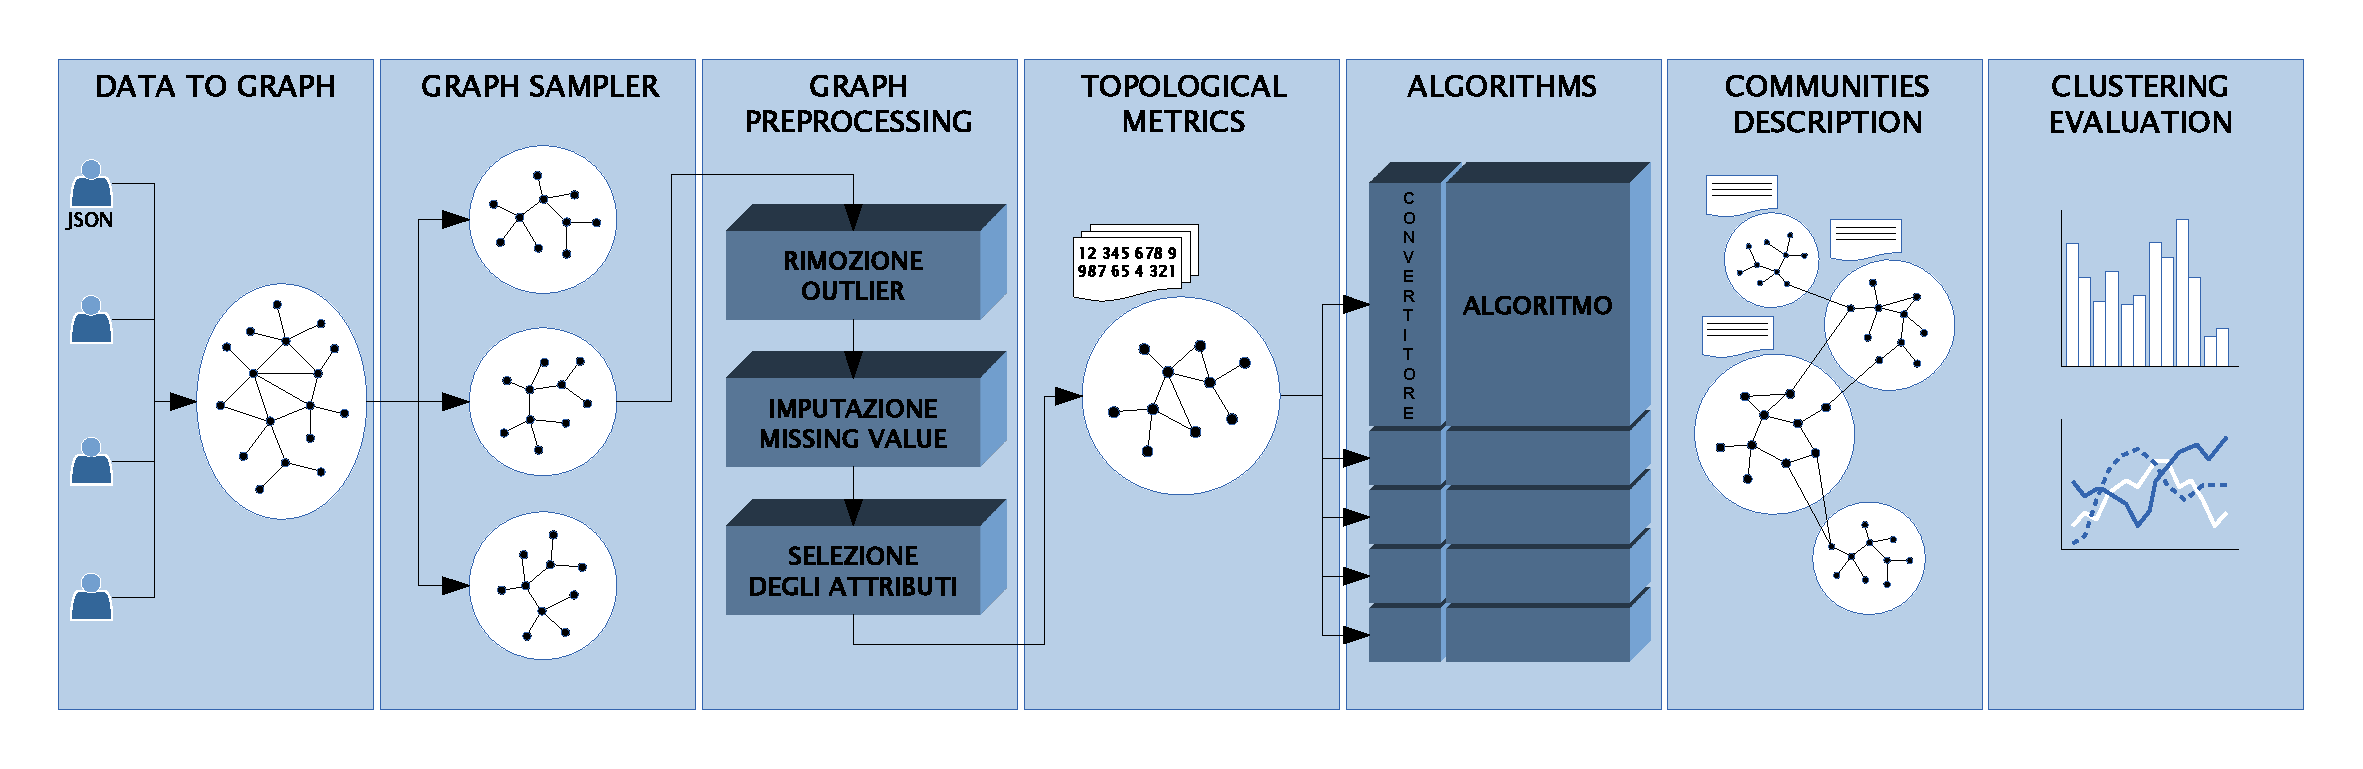
\includegraphics[width=1\textheight]{pictures/workflow.pdf}
    \caption{Workflow modulare dell'architettura}
    \label{fig:framework_flow}
\end{sidewaysfigure}

\chapter{Analisi dei risultati sperimentali}
\label{capitolo4}
\thispagestyle{empty}

In questo capitolo discutiamo i risultati degli algoritmi da noi selezionati sui dati raccolti.
\section{LAC}

\chapter{Conclusioni e sviluppi futuri}
\label{capitolo5}
\thispagestyle{empty}
%In quest'ultimo capitolo sintetizzeremo brevemente quanto � stato svolto nella tesi delineando le possibili prospettive future del lavoro, dall'integrazione di sorgenti di dati multiple (Facebook, Twitter e Foursquare) all'aggiunta di nuove funzionalit� utili al processo di segmentazione e al marketing in generale.

\section{Conclusioni}
Questo lavoro � stato motivato dall'esigenza di Neosperience---una azienda che offre servizi di marketing e \textit{customer experience}---di avere uno strumento per poter valorizzare i dati degli utenti raccolti tramite la piattaforma Engage: in particolare, l'obiettivo principale � quello di fornire delle tecniche di data preprocessing e degli algoritmi di clustering che siano di supporto alla segmentazione di mercato. La segmentazione di mercato � definita come quel processo che permette di partizionare un ampio insieme di clienti in piccoli gruppi (o \textit{segmenti}) caratterizzati da bisogni omogenei e simili comportamenti di acquisto. L'avvento dei Big Data � stato rivoluzionario in questo campo e ha modificato in maniera sostanziale l'approccio alla segmentazione di mercato. Se prima i dati di ogni consumatore erano difficilmente reperibili e comunque caratterizzati da un basso numero di attributi socio-demografici, con il paradigma dei Big Data si assiste a due fenomeni fondamentali: da un lato, � molto pi� semplice individuare i propri clienti grazie alla pervasivit� dei social network; dall'altro, ogni cliente � descritto da un elevato numero di attributi, come ad esempio i dati di profilo della propria pagina Facebook. Questa esplosione di informazioni rende pi� appetibile e potenzialmente pi� proficuo il processo di segmentazione, ma aggiunge, d'altro canto, un ulteriore livello di difficolt�. Gestire un grande insieme di clienti e individuare informazioni nascoste al suo interno diventa davvero difficoltoso senza l'ausilio di un procedimento automatico. � proprio a questo punto che la cluster analysis interviene a favore della segmentazione di mercato, fornendo una serie di strumenti che agevolano l'identificazione di caratteri emergenti dalla base di dati aziendale.\\
Purtroppo, complice la giovinezza della piattaforma Engage, non abbiamo potuto disporre dei profili utente su cui condurre tutti gli esperimenti necessari per svolgere il nostro lavoro. Il primo passo � stato, quindi, la creazione di una applicazione per la raccolta dei dati: abbiamo recuperato circa 25 mila profili Facebook, completi di numerose informazioni (anonimizzate) come l'et�, il genere, l'istruzione, gli interessi personali (le pagine su cui si � indicato \textit{like}) e relazioni di amicizia, creando un'unica rete sociale con attributi da cui sono partite le analisi e gli sviluppi principali del lavoro. Il passo successivo � stato quello di progettare e mettere a punto una infrastruttura per il preprocessing dei dati tramite procedure consolidate e di nuova generazione che tenessero conto delle peculiarit� delle reti sociali: con questi strumenti il grafo iniziale � stato pulito, trasformato e infine campionato in un insieme di sottografi con caratteristiche topologiche e di profilo molto variegate: in questa maniera, abbiamo potuto disporre di una serie di dataset su cui valutare, nel modo pi� oggettivo possibile, le varie tecniche di clustering. \\
Dopo un approfondito studio della letteratura, abbiamo selezionato un insieme di algoritmi progettando un'interfaccia di trasformazione tra i sottografi a disposizione e il formato in input di ogni algoritmo: in questo modo � stato possibile condurre dei test pratici che misurassero le prestazioni delle varie tecniche di clustering, individuando quelle pi� promettenti e isolando quelle insoddisfacenti. Per tale scopo sono stati valutati molteplici indici di qualit� ed i tempi d'esecuzione al variare dei parametri di ciascuna tecnica. In base a queste analisi abbiamo trovato metodi efficaci per il clustering di dataset medio-piccoli, altri computazionalmente pi� onerosi ma validi per il subspace clustering di grandi volumi di dati, nonch� algoritmi su grafi che sfruttano e ottimizzano simultaneamente le relazioni e la somiglianza tra gli individui, gestendo nativamente i valori mancanti e la dimensionalit� del problema. Infine, poich� ogni algoritmo richiede in ingresso almeno la specificazione del numero di cluster da individuare, abbiamo proposto delle soluzioni per la regolazione automatica dei parametri in input, delineando inoltre una serie di suggerimenti sugli scenari di successo e fallimento delle procedure a nostra disposizione. \\ 	

\section{Sviluppi futuri}
La naturale continuazione di questo lavoro pu� partire dalla soluzione di varie problematiche legate ai dati. Come gi� affermato nel Capitolo 3, la piattaforma Engage � alimentata da tre sorgenti di dati: Facebook, Twitter e Foursquare. In questa tesi abbiamo lavorato con i profili Facebook perch� l'informazione strutturata presente in essi ci ha permesso di focalizzare l'attenzione su aspetti pi� generali e specifici della cluster analysis. Integrare servizi come Twitter comporta, infatti, altrettante sfide: in questo contesto, il \textit{tweet} � l'informazione principale da analizzare e il suo carattere non strutturato impone l'utilizzo di sofisticate tecniche di elaborazione del linguaggio naturale per estrarre la semantica ad essi associata ed individuare gli interessi dell'utente. Un ulteriore obiettivo da raggiungere sarebbe quello dell'\textit{entity resolution}, ovvero l'identificazione e l'unificazione dei profili Facebook, Twitter e Foursquare che appartengono al medesimo individuo. Oltre alle difficolt� implementative di questa proposta ne incorrerebbero immediatamente altre teoriche, come l'esplosione della dimensionalit� dei dati e la formulazione di un modello coerente che tenga conto delle diversit� concettuali dei tre Social Network (si veda la \autoref{section_modello_dati}).\\

Un'altra prospettiva attraente riguarda l'automatizzazione della scelta dell'algoritmo: ci siamo chiesti, infatti, in che misura � possibile suggerire una tecnica di clustering su un certo dataset in ingresso, basandosi solamente sulle esecuzioni e le analisi fatte precedentemente, senza applicare tutti gli algoritmi a disposizione. Questo � un obiettivo tanto entusiasmante quanto delicato, infatti comporta una minuziosa attenzione a due questioni importanti: in primo luogo, come abbiamo sempre specificato nel corso del presente lavoro, un clustering � significativo solo se convalidato e, semmai, trasformato dal cliente; ci� comporta che se il framework suggerisce automaticamente l'utilizzo di un algoritmo con una certa parametrizzazione non vuol dire che il risultato sia da accettare in maniera \virgolette{dogmatica}. In secondo luogo, a complicare le cose, intervengono numerose sfide teoriche ed implementative. Se per il suggerimento di un algoritmo ci si vuole basare solamente sulle analisi fatte in precedenza, allora bisogna in qualche modo definire una misura di similarit� tra insiemi di individui, per associare al dataset in esame  il pi� simile dataset gi� processato e proporre per il primo le stesse considerazioni fatte sull'ultimo. Questo � un compito assai complicato sotto molteplici punti di vista. Sicuramente, per produrre risultati significativi � necessario aver memorizzato svariate analisi condotte su dataset altrettanto numerosi e il pi� possibile variegati dal punto di vista topologico e degli attributi di profilo. Conclusa questa fase resta comunque il problema della progettazione delle funzioni di similarit� tra dataset: come abbiamo affermato nei capitoli precedenti, il nostro lavoro mette  a disposizione un modulo per il calcolo di metriche topologiche che possono essere utilizzate per etichettare un grafo in ingresso e calcolare quanto esso si differenzi da quelli gi� processati. Per�, per raggiungere a pieno l'obiettivo � necessario stabilire anche in quale misura due dataset sono simili relativamente agli attributi e individuare, in definitiva, una funzione univoca che tenga conto contemporaneamente delle caratteristiche topologiche e di profilo dei dati in ingresso.\\

Sempre nell'ambito del marketing e delle dinamiche \textit{social} potrebbe essere molto interessante arricchire il nostro lavoro con strumenti di \textit{sentiment analysis} che svolgono oramai un ruolo di fondamentale importanza per recuperare automaticamente le opinioni dei clienti riguardo un prodotto o servizio. Utilizzando queste tecniche � possibile condurre una ulteriore segmentazione di mercato mirata ad intercettare il \textit{mood} dei consumatori e intervenire a seconda della positivit� o negativit� delle opinioni e del relativo grado di intensit� emotiva. Questi aspetti possono avere ancor pi� valore del singolo \textit{like} sulla pagina Facebook aziendale, e rappresentano per tanto una nuova frontiera per il monitoraggio della reputazione del brand e la pianificazione di innovative strategie di marketing.\\

In ultimo, citiamo una idea stimolante riguardo il \textit{viral marketing} che pu� essere facilmente integrata nel nostro progetto. Supponiamo che una azienda stia cercando di promuovere un prodotto all'interno di una popolazione di potenziali clienti tramite l'offerta di campioni di prova gratuiti: � fondamentale chiedersi a chi proporre questa offerta. Gli studi sul \textit{marketing virale} \cite{WOM} affermano che c'� un vantaggio molto importante nel far conoscere un certo brand tramite il \textit{passaparola} tra conoscenti: infatti un consumatore � pi� propenso all'acquisto se � stato consigliato da una persona fidata. Questo meccanismo, inoltre, innesca una cascata di segnalazioni che da un numero basso di utilizzatori iniziali pu� portare ad un ampio gruppo di clienti finali. Per questa ragione � essenziale individuare, all'interno di un grafo sociale, gli \textit{opinion leader}, ovvero le persone pi� influenti dalle quali � possibile ottenere l'effetto cascata maggiore e proporre loro l'offerta dei campioni gratuiti \cite{InfluNodes}.
\chapter{Realizzazioni sperimentali e valutazione}
\label{capitolo6}
\thispagestyle{empty}

\begin{quotation}
{\footnotesize
\noindent\emph{``Bambino: Questo � l'ultimo avviso per voi e i vostri rubagalline \\
Il pistolero si alza: Che avete detto? \\
Bambino: RUBAGALLINE \\
Il pistolero si risiede: Aaah.''}
\begin{flushright}
Lo chiamavano Trinit\`a \dots
\end{flushright}
}
\end{quotation}
\vspace{0.5cm}

\noindent Si mostra il progetto dal punto di vista sperimentale, le cose materialmente realizzate. In questa sezione si mostrano le attivit\`a sperimentali svolte, si illustra il funzionamento del sistema (a grandi linee) e si spiegano i risultati ottenuti con la loro valutazione critica. Bisogna introdurre dati sulla complessit\`a degli algoritmi e valutare l'efficienza del sistema.
\chapter{Direzioni future di ricerca e conclusioni}
\label{capitolo7}
\thispagestyle{empty}

\begin{quotation}
{\footnotesize
\noindent\emph{``Terence: Mi fai un gelato anche a me? Lo vorrei di pistacchio. \\
Bud: Non ce l'ho il pistacchio. C'ho la vaniglia, cioccolato, fragola, limone e caff\'e. \\
Terence: Ah bene. Allora fammi un cono di vaniglia e di pistacchio. \\
Bud: No, non ce l'ho il pistacchio. C'ho la vaniglia, cioccolato, fragola, limone e caff\'e. \\
Terence: Ah, va bene. Allora vediamo un po', fammelo al cioccolato, tutto coperto di pistacchio. \\
Bud: Ehi, macch� sei sordo? Ti ho detto che il pistacchio non ce l'ho! \\
Terence: Ok ok, non c'� bisogno che t'arrabbi, no? Insomma, di che ce l'hai? \\
Bud: Ce l'ho di vaniglia, cioccolato, fragola, limone e caff\'e! \\
Terence: Ah, ho capito. Allora fammene uno misto: mettici la fragola, il cioccolato, la vaniglia, il limone e il caff\'e. Charlie, mi raccomando il pistacchio, eh.''}
\begin{flushright}
Pari e dispari
\end{flushright}
}
\end{quotation}
\vspace{0.5cm}

\noindent Si mostrano le prospettive future di ricerca nell'area dove si \`e svolto il lavoro. Talvolta questa sezione pu\`o essere l'ultima sottosezione della precedente. Nelle conclusioni si deve richiamare l'area, lo scopo della tesi, cosa \`e stato fatto,come si valuta quello che si \`e fatto e si enfatizzano le prospettive future per mostrare come andare avanti nell'area di studio.

\cleardoublepage
% ---- Bibliography ----
\addcontentsline{toc}{chapter}{Bibliografia}
\bibliographystyle{plain}
\bibliography{bibl_tesi}
\nocite{*}

\appendix

\pagestyle{fancy} 
\fancyfoot{}                                               
\renewcommand{\chaptermark}[1]{\markboth{\appendixname\ \thechapter.\ #1}{}} 
\renewcommand{\sectionmark}[1]{\markright{\thesection.\ #1}}         
\fancyhead[LE,RO]{\bfseries\thepage}    
                                        
\fancyhead[RE]{\bfseries\leftmark}    
\fancyhead[LO]{\bfseries\rightmark}     
\renewcommand{\headrulewidth}{0.3pt} 

%\chapter{Missing Values}
\label{missing_values}
\thispagestyle{empty}

A ciascun utente sono associati due tipi di proprietà: il profilo e i like. I like sono ovviamente variabili da un individuo all'altro, né a senso trattare l'assenza di un \textit{mi piace} su un certo contenuto come valore mancante. In generale, parliamo quindi di valori mancanti solo per i dati di profilo, dove sono raccolte le informazioni biografiche dell'utente. Una ulteriore ragione per dare maggior peso all'assenza di informazione di profilo rispetto ai like è il ruolo che questi dati rivestiranno nell'analisi. Mentre i like sono fondamentali per produrre il clustering, gli attributi di profilo sono essenziali per interpretare i cluster. Una volta tracciati i cluster siamo in grado di capire quali interessi accomunano le persone; ma, assumendo di non avere altre fonti di informazione, senza i dati del profilo non è possibile caratterizzare questi gruppi, descrivere con le variabili della segmentazione tradizionale le persone che ne fanno parte, ed il risultato perde significativamente valore.\\
Tra gli algoritmi che abbiamo selezionato, solo Cesna \cite{cesna} è insensibile ai valori mancanti; per tutti gli altri è stato necessario produrre una versione completa dei dati. \`E tuttavia necessario provare a intuire la causa dell'assenza dei dati per stabilire quale meccanismo di completamento dell'informazione ne accresca, e non riduca, la qualità. In questa fase, abbiamo fatto ricorso a tre soluzioni: rimuovere l'individuo con missing values (la riga del dataset), rimuovere integralmente l'attributo (la colonna del dataset) o inferire il valore laddove assente. La prima soluzione è consigliabile quando l'individuo è così povero di informazione da non produrre alcun beneficio all'analisi. Le cause di tale penuria sono disparate: un profilo sostanzialmente inattivo, non aggiornato né mantenuto dal momento della creazione; l'irrilevanza dell'informazione nell'ottica del proprietario del profilo; la riservatezza, tale che o l'utente non ha appositamente inserito l'informazione nel profilo o i permessi in nostro possesso non sono sufficienti per accedere ai dati esistenti. Richiamando la terminologia introdotta in \autoref{subsec:missing_value}, inattività e irrilevanza ricadono nella tipologia MCAR, in quanto non vi è alcuna connessione tra il valore dell'attributo mancante e il fatto che non sia stato inserito. La riservatezza invece è generalmente MNAR; sebbene un individuo preoccupato per la propria privacy possa essere portato a occultare indiscriminatamente i propri dati (MCAR), è ragionevole e conservativo assumere che il non pubblicare una informazione possa dipendere dal valore dell'attributo per l'utente considerato. Per meglio comprendere i dati che avevamo raccolto e discriminare tra questi due casi, abbiamo studiato la relazione nel dataset tra la completezza dei dati biografici e il numero di like, assumendo quest'ultimo come una misura della partecipazione dell'utente al social network e dell'attività del profilo; i risultati sono mostrati in \autoref{fig:profile_vs_likes}. L'ipotesi alla base di questo studio, da confermare o smentire, è che un profilo povero di informazione sia anche poco attivo, quindi povero di like.
\begin{figure}[h]
    \centering
    \begin{subfigure}[b]{0.47\textwidth}
		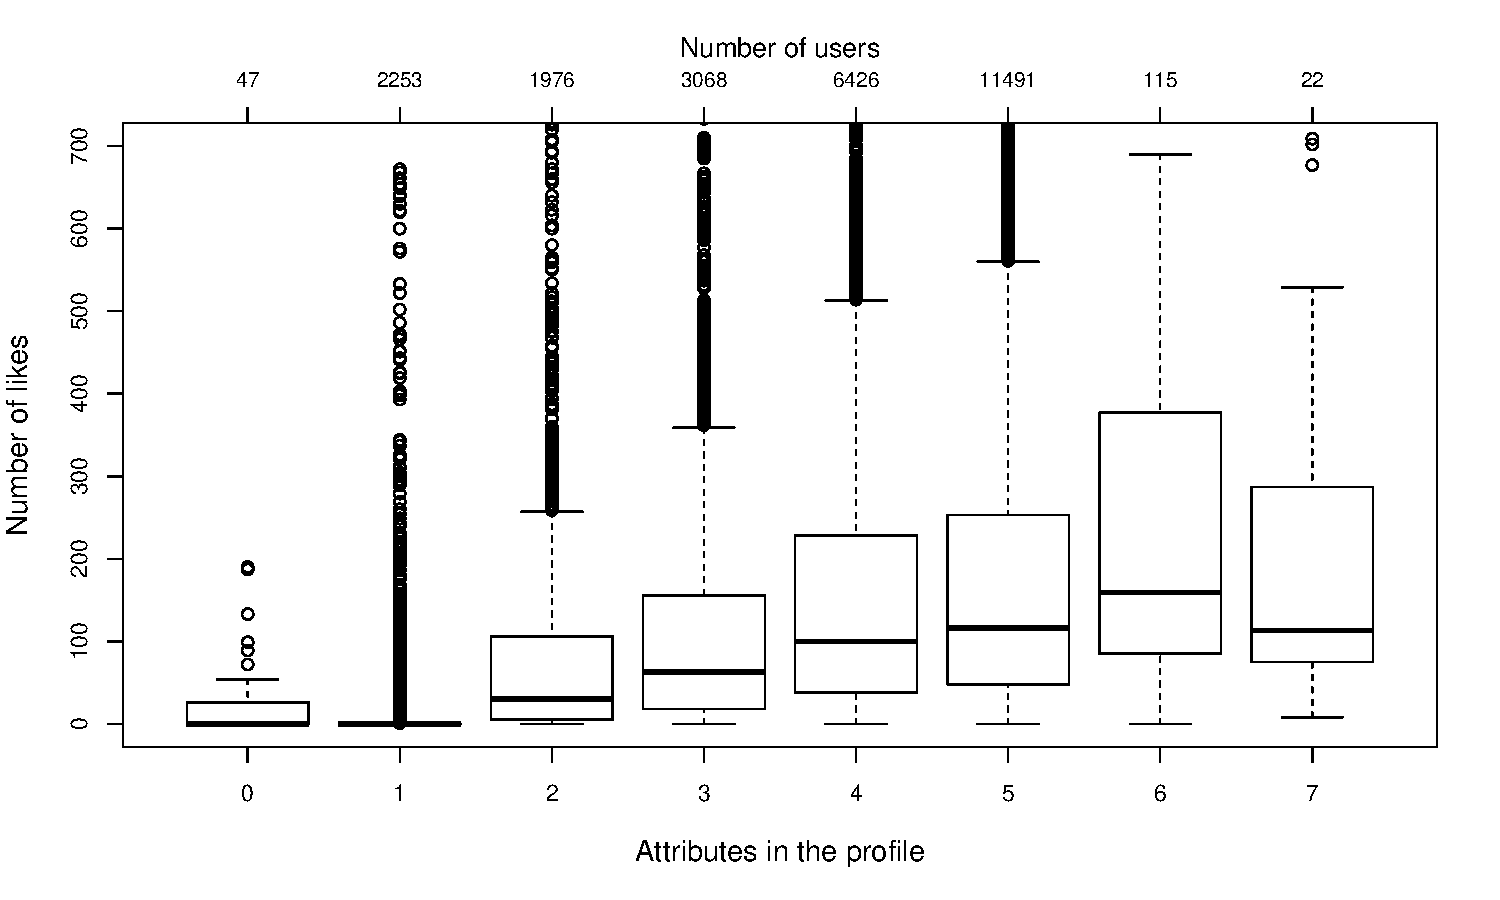
\includegraphics[width=\textwidth]{pictures/profile_vs_likes.pdf}
		\caption{dataset completo}
		\label{fig:profile_vs_likes_users}
	\end{subfigure}
	\hfill
    %add desired spacing between images, e. g. ~, \quad, \qquad, \hfill etc.
    %(or a blank line to force the subfigure onto a new line)
	\begin{subfigure}[b]{0.47\textwidth}
		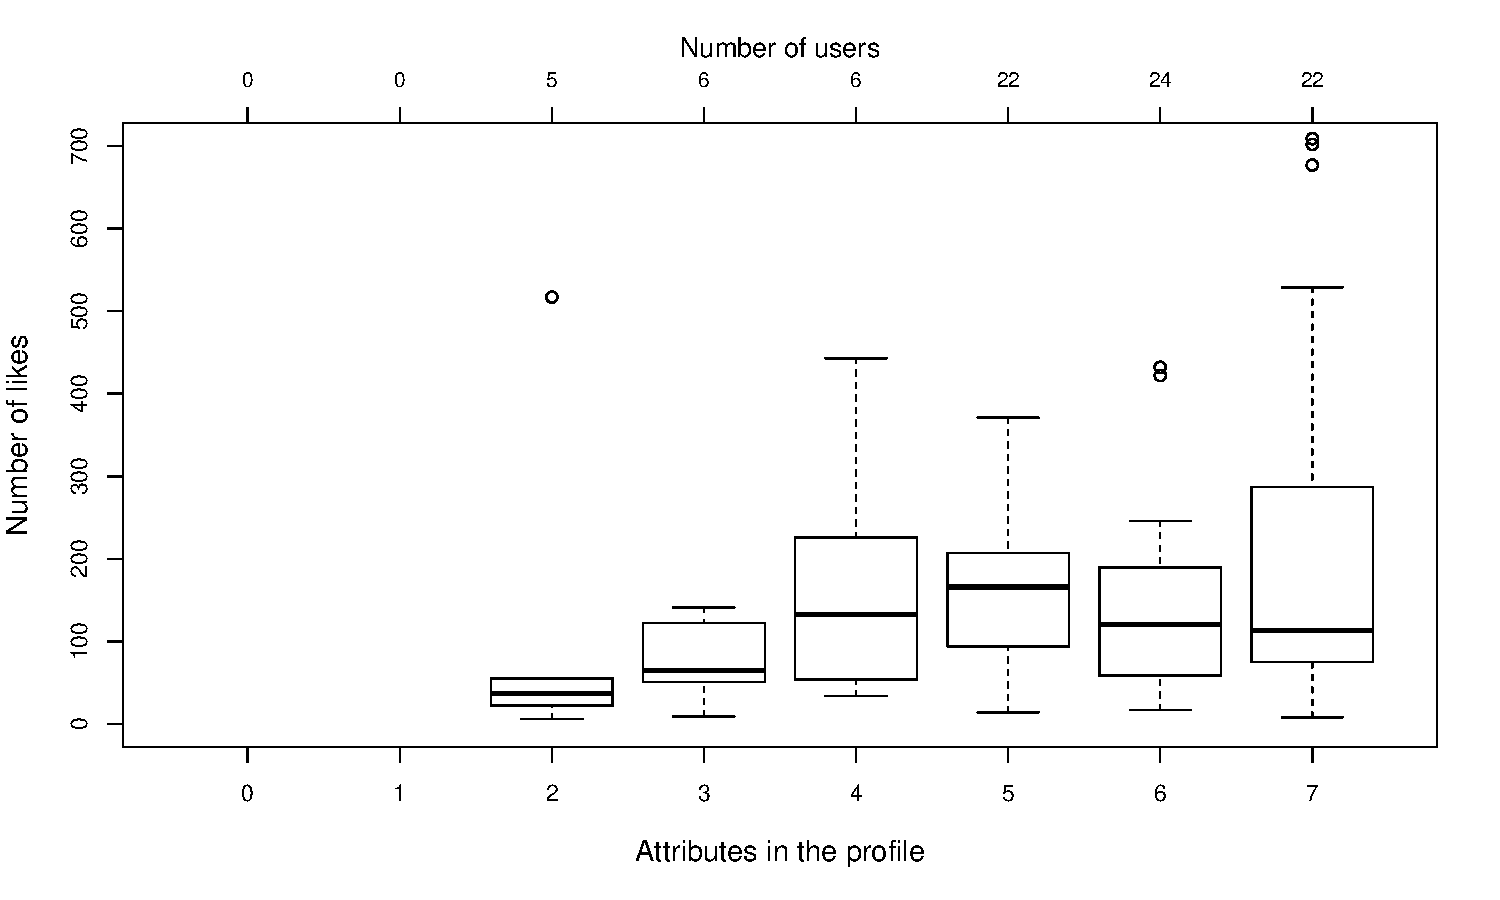
\includegraphics[width=\textwidth]{pictures/profile_vs_likes_dau.pdf}
		\caption{utenti dell'applicazione facebook}
		\label{fig:profile_vs_likes_daus}
	\end{subfigure}
	\caption{Relazione tra il numero di attributi e like nel profilo utente}
	\label{fig:profile_vs_likes}
\end{figure}\\
A sinistra (\autoref{fig:profile_vs_likes_users}), la relazione è valutata sull'intera popolazione; a destra sui soli utenti dell'applicazione. Sulle ascisse riportiamo il numero di attributi specificati dall'utente: da 0, profilo completamente vuoto, a 7\footnote{Sebbene il profilo contenga effettivamente nove attributi, abbiamo accorpato i tre campi (opzionali) relativi all'educazione in un unico attributo, assente se nessuno dei tre gradi di istruzione è specificato}, informazione piena. Si può osservare che esiste una moderata correlazione tra le grandezze sugli assi, la completezza del profilo e il numero di like, che crescono di pari passo. Fa eccezione l'ultima colonna, che tuttavia contiene solo utenti dell'applicazione ed è infatti identica nei due grafici. La differenza è che solo per questi ultimi, gli utenti dell'applicazione, siamo certi di osservare il profilo completo di ogni informazione inserita, a prescindere dalle impostazioni di visibilità. Per tutti gli altri utenti infatti la quantità di informazione che possiamo osservare dipende dai permessi concessi all'utente che li ha aggiungi al grafo (vedi liste di amici).
Data la vastità del dataset, oltre 25000 nodi, è estremamente inverosimile che nessuno tra gli utenti che non hanno partecipato alla raccolta dei dati abbia un profilo completo, e possiamo quindi percepire i limiti dell'informazione indiretta. Si aggiunge pertanto un'altra causa di assenza dei dati, legata stavolta al punto di vista dal quale osserviamo il grafo sociale. Questa connessione tra i due aspetti del profilo ci ha permesso di rimuovere gli utenti sostanzialmente privi di dati biografici senza degradare l'informazione complessiva nel dataset.\\
La seconda soluzione, rimuovere integralmente una dimensione, è necessaria quando l'attributo è mancante per una significativa porzione della popolazione: in questo scenario, rimuovere gli individui privi dell'attributo sarebbe un spreco di informazione e non è nemmeno disponibile sufficiente informazione reale per inferire i valori mancanti. Dai risultati in \autoref{table:missing_values} si evince che gli attributi \textit{orientamento sessuale} e \textit{stato sentimentale} sono specificati da una estrema minoranza di utenti, certamente troppo pochi per applicare una procedura di imputazione; pertanto sono stati rimossi dal dataset.
\begin{table}[h]
\resizebox{0.8\textwidth}{!}{\begin{minipage}{\textwidth}
\begin{tabular}{| c | c | c | c | c | c | c | r}
\multicolumn{1}{c}{genere}
 &  \multicolumn{1}{c}{età}
 & \multicolumn{1}{c}{\specialcell[t]{luogo di\\nascita}}
 & \multicolumn{1}{c}{\specialcell[t]{luogo di\\residenza}}
 & \multicolumn{1}{c}{educazione}
 & \multicolumn{1}{c}{\specialcell[t]{orientamento\\sessuale}}
 & \multicolumn{1}{c}{\specialcell[t]{stato\\sentimentale}}
 & \multicolumn{1}{c}{}
 \tabularnewline
\cline{1-7}
0.0078 & 0.3253 & 0.2802 & 0.2364 & 0.2429 & 0.9913 & 0.9984 & dataset\tabularnewline
\cline{1-7}
0 & 0 & 0.2 & 0.1882 & 0.1412 & 0.5412 & 0.5186 & DAU\tabularnewline
\cline{1-7}
\end{tabular}
\caption{Distribuzione dei valori mancanti per attributo}
\label{table:missing_values}
\end{minipage} }
\end{table}
Una analisi a parte merita l'educazione, che descrive l'aver frequentato la scuola superiore, un corso universitario triennale e magistrale. Nonostante si tratti di campi opzionali---un individuo può certamente non aver frequentato l'università---e il valore si assesti ben al di sotto della media italiana\footnote{Dal Quarto Rapporto sulla coesione sociale in Italia, il 37.8\% dei giovani tra i 18 e 24 anni ha conseguito al massimo la licenza media}, poiché i nostri dati descrivono principalmente studenti universitari e la loro cerchia di  amici, risulta inspiegata una percentuale tanto alta di assenza di qualsivoglia livello di istruzione superiore (\autoref{table:missing_values}). Questo lascia pensare che vi sia un significativa incidenza di missing values anche per questo attributo, ed un stima per difetto si ottiene dall'incidenza dei dati incongruenti: individui che frequentano studi universitari senza aver inserito nel proprio profilo i gradi di istruzione inferiori (\autoref{table:missing_values_education}).
\begin{table}[h]
\resizebox{0.8\textwidth}{!}{\begin{minipage}{\textwidth}
\begin{tabular}{l | c | c | c | r}
 \multicolumn{1}{c}{} 
 & \multicolumn{1}{c}{scuola superiore}
 & \multicolumn{1}{c}{università triennale}
 & \multicolumn{1}{c}{università specialistica}
 & \multicolumn{1}{c}{}
 \tabularnewline
\cline{2-4}
\multirow{2}{*}{\centering dataset} & 0.3232 & 0.4176 & 0.9297 & non specificato \tabularnewline
\cline{2-4}
& 0.0794 & 0.0120 & 0 & incongruente \tabularnewline
\cline{2-4}
\cline{2-4}
\multirow{2}{*}{\centering DAU} & 0.2824 & 0.2 & 0.8353 & non specificato \tabularnewline
\cline{2-4}
& 0.1412 & 0 & 0 & incongruente \tabularnewline
\cline{2-4}
\end{tabular}
\caption{Distribuzione dei valori mancanti per ciascun grado di istruzione}
\label{table:missing_values_education}
\end{minipage} }
\end{table}\\
Ad esempio, l'attributo \textit{scuola superiore} è assente dal 28\% dei profili degli utenti che hanno utilizzato la nostra applicazione, ma ben la metà di questi hanno pubblicato la frequenza di corsi universitari pur senza citare quelli precedenti.\\
In ultimo, i valori possono essere dedotti tramite imputazione. Come discusso precedentemente, i dati mancanti sono anche MNAR e per essi non esiste una procedura univoca di inferenza. Abbiamo deciso pertanto di sviluppare una procedura di imputazione ad hoc, facendo leva sull'omofilia nella rete. Per ciascun individuo con missing value abbiamo considerato gli utenti a cui è connesso nel grafo delle amicizie, e stimato il valore dell'attributo mancante da quello dei suoi vicini. A questo punto, la stima può avvenire con uno dei metodi definiti in letteratura: media, hot-deck, regressione etc. Un problema di questo metodo è che non sfrutta tutta l'informazione nel dataset per completare i valori mancanti ma si avvale soltanto dei vicini. Quando un individuo non ha un vicinato sufficientemente ampio, o i vicini a loro volta non possiedono l'attributo mancante nel soggetto, l'imputazione non ha basi sufficientemente solide per essere affidabile. Per questa ragione abbiamo ulteriormente rimosso dal dataset i nodi poveri di attributi di profilo e debolmente connessi al grafo. Con le due fasi di rimozione dei dati impuri, la dimensione del dataset è drasticamente calata; abbiamo quantificato la perdita di informazione in \autoref{table:cleaned_dataset_statistics}.
\begin{table}[h]
\centering
\begin{tabular}{l | c | c | c |}
 \multicolumn{1}{c}{} 
 & \multicolumn{1}{c}{nodi}
 & \multicolumn{1}{c}{archi \textit{friend}}
 & \multicolumn{1}{c}{archi \textit{like}}
 \tabularnewline
\cline{2-4}
originale (con MV) & 25853 & 975\hspace{2pt}382 & 4\hspace{2pt}391\hspace{2pt}494 \tabularnewline
\cline{2-4}
completo (senza MV) & 16336 & 710\hspace{2pt}711 & 3\hspace{2pt}131\hspace{2pt}019 \tabularnewline
\cline{1-4}
decremento assoluto & 9517 & 264\hspace{2pt}671 & 1\hspace{2pt}260\hspace{2pt}475 \tabularnewline
\cline{2-4}
decremento percentuale & 36.81\% & 27.14\% & 28.7\% \tabularnewline
\cline{2-4}
\end{tabular}
\caption{Perdita di informazione durante l'imputazione dei valori mancanti}
\label{table:cleaned_dataset_statistics}
\end{table}\\
%Missingness by attribute
%interested_in 0.9913379
%gender 0.007874636
%hometown 0.280652
%location 0.2375384
%birthday 0.3262855
%relationship_status 0.9983857
%education 0.2437594
%missingness for education
%HS			College		GR Sc		
%0.3231751 	0.4175526 	0.9296795
%True missing
%HS			College		GR Sc
%0.0794157	0.01204819	0
missing values introduced by transformations (coordinates missing after geocoding)
%\chapter{Analisi dei dati}
\label{appendiceB}
\thispagestyle{empty}

\begin{table}[h]
\small
\centering
\begin{tabular}{l | c | c | c | c |}
 \multicolumn{1}{c}{} 
 & \multicolumn{1}{c}{utenti}
 & \multicolumn{1}{c}{archi \textit{friend}}
 & \multicolumn{1}{c}{\textit{like}}
 & \multicolumn{1}{c}{componenti}
 \tabularnewline
\cline{2-5}
1 & 1258 & 70\hspace{2pt}967 & 112\hspace{2pt}707 & 1 \tabularnewline
\cline{2-5}
2 & 1419 & 27\hspace{2pt}399 & 111\hspace{2pt}684 & 3 \tabularnewline
\cline{2-5}
3 & 1390 & 18\hspace{2pt}469 & 106\hspace{2pt}785 & 2 \tabularnewline
\cline{2-5}
4 & 1565 & 88\hspace{2pt}789 & 125\hspace{2pt}916 & 2 \tabularnewline
\cline{2-5}
5 & 1469 & 48\hspace{2pt}023 & 139\hspace{2pt}691 & 2 \tabularnewline
\cline{2-5}
6 & 1461 & 19\hspace{2pt}117 & 121\hspace{2pt}544 & 2 \tabularnewline
\cline{2-5}
7 & 1579 & 52\hspace{2pt}330 & 124\hspace{2pt}374 & 3 \tabularnewline
\cline{2-5}
8 & 1250 & 32\hspace{2pt}134 & 104\hspace{2pt}848 & 3 \tabularnewline
\cline{2-5}
9 & 3091 & 115\hspace{2pt}695 & 222\hspace{2pt}839 & 4 \tabularnewline
\cline{2-5}
10 & 3143 & 85\hspace{2pt}396 & 223\hspace{2pt}146 & 2 \tabularnewline
\cline{2-5}
11 & 2633 & 56\hspace{2pt}785 & 195\hspace{2pt}395 & 4 \tabularnewline
\cline{2-5}
12 & 2951 & 110\hspace{2pt}737 & 197\hspace{2pt}220 & 2 \tabularnewline
\cline{2-5}
13 & 3166 & 61\hspace{2pt}634 & 204\hspace{2pt}507 & 2 \tabularnewline
\cline{2-5}
14 & 2633 & 107\hspace{2pt}249 & 208\hspace{2pt}152 & 1 \tabularnewline
\cline{2-5}
15 & 2997 & 90\hspace{2pt}389 & 191\hspace{2pt}949 & 1 \tabularnewline
\cline{2-5}
16 & 3133 & 153\hspace{2pt}498 & 225\hspace{2pt}844 & 1 \tabularnewline
\cline{2-5}
17 & 5690 & 147\hspace{2pt}368 & 340\hspace{2pt}145 & 1 \tabularnewline
\cline{2-5}
18 & 5081 & 160\hspace{2pt}955 & 307\hspace{2pt}814 & 3 \tabularnewline
\cline{2-5}
19 & 6398 & 426\hspace{2pt}429 & 353\hspace{2pt}303 & 3 \tabularnewline
\cline{2-5}
20 & 5923 & 293\hspace{2pt}638 & 338\hspace{2pt}710 & 2 \tabularnewline
\cline{2-5}
21 & 5966 & 288\hspace{2pt}784 & 340\hspace{2pt}986 & 1 \tabularnewline
\cline{2-5}
22 & 5662 & 151\hspace{2pt}093 & 323\hspace{2pt}894 & 1 \tabularnewline
\cline{2-5}
23 & 10880 & 472\hspace{2pt}228 & 533\hspace{2pt}653 & 2 \tabularnewline
\cline{2-5}
24 & 11073 & 489\hspace{2pt}630 & 542\hspace{2pt}150 & 1 \tabularnewline
\cline{2-5}
25 & 10730 & 413\hspace{2pt}476 & 550\hspace{2pt}188 & 2 \tabularnewline
\cline{2-5}
26 & 10839 & 484\hspace{2pt}518 & 538\hspace{2pt}002 & 1 \tabularnewline
\cline{2-5}
\end{tabular}
\caption{Propriet� dei campioni del dataset}
\label{table:sample_stats}
\end{table}

\begin{table}[h]
\small
\centering
\begin{tabular}{l | c | c | c | c | c | c | c | c |}
\cline{2-9}
1 & 1 & 0.053 & 0.021 & 0.127 & 0.163 & 0.016 & 0.067 & 0.056 \tabularnewline
\cline{2-9}
2 &  & 1 & 0.031 & 0.115 & 0.057 & 0.073 & 0.104 & 0.036 \tabularnewline
\cline{2-9}
3 &  &  & 1 & 0.03 & 0.058 & 0.032 & 0.055 & 0.053 \tabularnewline
\cline{2-9}
4 &  &  &  & 1 & 0.079 & 0.105 & 0.114 & 0.085 \tabularnewline
\cline{2-9}
5 &  &  &  &  & 1 & 0.019 & 0.042 & 0.027 \tabularnewline
\cline{2-9}
6 &  &  &  &  &  & 1 & 0.029 & 0.045 \tabularnewline
\cline{2-9}
7 &  &  &  &  &  &  & 1 & 0.048 \tabularnewline
\cline{2-9}
8 &  &  &  &  &  &  &  & 1 \tabularnewline
\cline{2-9}
\end{tabular}
\caption{Omogeneit\`a tra i campioni di 1500 nodi del dataset}
\label{table:omogeneita_1500}
\end{table}
%\chapter{Listato}
\label{appendiceC}
\thispagestyle{empty}

\noindent Il listato (o solo parti rilevanti di questo, se risulta particolarmente esteso) con l'autodocumentazione relativa.
%\chapter{Il manuale utente}
\label{appendiceD}
\thispagestyle{empty}

\noindent Manuale utente per l'utilizzo del sistema
%\chapter{Esempio di impiego}
\label{appendiceE}
\thispagestyle{empty}

\noindent Un esempio di impiego del sistema realizzato.
%\chapter{Datasheet}
\label{appendiceF}
\thispagestyle{empty}

\noindent Eventuali Datasheet di riferimento.

\end{document}





